%%%%%%%%%%%%%%%%%%%%%%%%%%%%%%%%%%%%%%%%%%%%%%%%%%%%%%%%%%%%%%%%%%%%%%%%%%%%
%% Author template for Management Science (mnsc) for articles with no e-companion (EC)
%% Mirko Janc, Ph.D., INFORMS, mirko.janc@informs.org
%% ver. 0.95, December 2010
%%%%%%%%%%%%%%%%%%%%%%%%%%%%%%%%%%%%%%%%%%%%%%%%%%%%%%%%%%%%%%%%%%%%%%%%%%%%
\documentclass[mnsc,blindrev]{informs3}
%\documentclass[mnsc,nonblindrev]{informs3} % current default for manuscript submission

\OneAndAHalfSpacedXI
%%\OneAndAHalfSpacedXII % Current default line spacing
%%\DoubleSpacedXII
%%\DoubleSpacedXI

% If hyperref is used, dvi-to-ps driver of choice must be declared as
%   an additional option to the \documentclass. For example
%\documentclass[dvips,mnsc]{informs3}      % if dvips is used
%\documentclass[dvipsone,mnsc]{informs3}   % if dvipsone is used, etc.

% Private macros here (check that there is no clash with the style)

%https://tex.stackexchange.com/questions/400692/different-height-of-tikz-subfigures-despite-same-axis-width-height

\usepackage{booktabs}
\usepackage{tabularx}
\usepackage{colortbl}
\usepackage{array}
\usepackage{multirow,calc,amsmath}
\newlength\mylenA
\newlength\mylenB
\newlength\mylenC
\newlength\mylenD
\usepackage{tikz}
\usepackage{tcolorbox}
\usepackage{etoolbox}
\AtBeginEnvironment{tcolorbox}{\normalsize}

\usepackage{adjustbox}[valign=t]

\tcbuselibrary{skins, breakable}

\makeatletter
\tcbset{
  tabular/.style={
    boxsep=\z@,top=\z@,bottom=\z@,leftupper=\z@,rightupper=\z@,
    toptitle=1mm,bottomtitle=1mm,boxrule=0.5mm,
    fontupper=\small,
    before upper={\arrayrulecolor{tcbcolframe}\def\arraystretch{1.1}%
      \tcb@hack@currenvir\tabular{#1}},
    after upper=\endtabular\arrayrulecolor{black}},
}
\makeatother

\usepackage{color, colortbl}
\usepackage{graphicx}
%\usepackage{subfigure}
\usepackage{caption}
\usepackage{subcaption}
%\usepackage{tcolorbox}
\usepackage{physics}
\usepackage{dsfont}
\usepackage{booktabs}
\usepackage{amsmath}
\usepackage{amsthm}
\usepackage{hyperref}
\usepackage{makecell}
\usepackage{tikz}
\usepackage{pgfplots}
\usepackage{tikzviolinplots}
\usepgfplotslibrary{external}
\tikzexternalize
\usepackage{minted}
\usemintedstyle{gruvbox-light}
\usepackage{scontents}
\usepackage{statmath}

 
\renewcommand\theadalign{bc}
\renewcommand\theadfont{\bfseries}
\renewcommand\theadgape{\Gape[4pt]}
\renewcommand\cellgape{\Gape[4pt]}

\newcommand{\gray}{\rowcolor[gray]{.90}}
% Natbib setup for author-year style
\usepackage{natbib}
 \bibpunct[, ]{(}{)}{,}{a}{}{,}%
 \def\bibfont{\small}%
 \def\bibsep{\smallskipamount}%
 \def\bibhang{24pt}%
 \def\newblock{\ }%
 \def\BIBand{and}%
\def\pipeline{prediction insight pipeline}
\newcommand{\tw}[1]{\textcolor{red}{Tong: #1}}

\def\checkmark{\tikz\fill[scale=0.4](0,.35) -- (.25,0) -- (1,.7) -- (.25,.15) -- cycle;} 

% \newtheorem{theorem}{Theorem}
% \newtheorem{corollary}{Corollary}[theorem]
% \newtheorem{lemma}[theorem]{Lemma}
% \newtheorem{remark}{Remark}
% \newtheorem{proof}{Proof}


%% Setup of theorem styles. Outcomment only one.
%% Preferred default is the first option.
\TheoremsNumberedThrough     % Preferred (Theorem 1, Lemma 1, Theorem 2)
%\TheoremsNumberedByChapter  % (Theorem 1.1, Lema 1.1, Theorem 1.2)
\ECRepeatTheorems

%% Setup of the equation numbering system. Outcomment only one.
%% Preferred default is the first option.
\EquationsNumberedThrough    % Default: (1), (2), ...
%\EquationsNumberedBySection % (1.1), (1.2), ...

% For new submissions, leave this number blank.
% For revisions, input the manuscript number assigned by the on-line
% system along with a suffix ".Rx" where x is the revision number.
\MANUSCRIPTNO{MS-0001-1922.65}

%%%%%%%%%%%%%%%%
\begin{document}
%%%%%%%%%%%%%%%%

% Outcomment only when entries are known. Otherwise leave as is and
%   default values will be used.
%\setcounter{page}{1}
%\VOLUME{00}%
%\NO{0}%
%\MONTH{Xxxxx}% (month or a similar seasonal id)
%\YEAR{0000}% e.g., 2005
%\FIRSTPAGE{000}%
%\LASTPAGE{000}%
%\SHORTYEAR{00}% shortened year (two-digit)
%\ISSUE{0000} %
%\LONGFIRSTPAGE{0001} %
%\DOI{10.1287/xxxx.0000.0000}%

% Author's names for the running heads
% Sample depending on the number of authors;
% \RUNAUTHOR{Jones}
% \RUNAUTHOR{Jones and Wilson}
% \RUNAUTHOR{Jones, Miller, and Wilson}
% \RUNAUTHOR{Jones et al.} % for four or more authors
% Enter authors following the given pattern:
%\RUNAUTHOR{}

% Title or shortened title suitable for running heads. Sample:
% \RUNTITLE{Bundling Information Goods of Decreasing Value}
% Enter the (shortened) title:
\RUNTITLE{The Illusion of Interpretation}

% Full title. Sample:
% \TITLE{Bundling Information Goods of Decreasing Value}
% Enter the full title:
%change title!!!
\TITLE{The Illusion of Interpretation: Post Hoc Explanations Aren't a Silver Bullet for Business Research}

% Block of authors and their affiliations starts here:
% NOTE: Authors with same affiliation, if the order of authors allows,
%   should be entered in ONE field, separated by a comma.
%   \EMAIL field can be repeated if more than one author
\ARTICLEAUTHORS{%
\AUTHOR{Snidely Slippery}
\AFF{Department of Bread Spread Engineering, Dairy University, Cowtown, IL 60208, \EMAIL{slippery@dairy.edu}} %, \URL{}}
\AUTHOR{Marg Arinella}
\AFF{Institute for Food Adulteration, University of Food Plains, Food Plains, MN 55599, \EMAIL{m.arinella@adult.ufp.edu}}
% Enter all authors
} % end of the block

% palette for colorblindness https://davidmathlogic.com/colorblind/#%23000000-%23E69F00-%2356B4E9-%23009E73-%23F0E442-%230072B2-%23D55E00-%23CC79A7

\ABSTRACT{%
In the realm of business research, the need to demystify black-box machine learning models is paramount. Post hoc explanation methods, such as LIME and SHAP, have gained widespread popularity for this purpose. Common practice involves constructing a black-box model and subsequently employing these post hoc tools to interpret the model's output. However, this approach has fundamental flaws. This paper delves into the potential misleading effects of post hoc explainers when used to interpret phenomena underlying a model's training data, in particular estimating the $\beta$ of a linear representation of the ground truth feature importance. Our study focuses on what we term the ``Prediction Insight Pipeline" in business research, where we identify and illustrate critical issues. We reveal that post hoc explanations not only often deviate from the actual truths in the data but also display inconsistency among themselves, further muddling the understanding of these models. To address these challenges, we introduce and evaluate straightforward and intuitive mitigation strategies. These strategies form a basis for explorations of how to maximize the faithfulness of post hoc explanations. We test our strategies on both simulated and real datasets. Our three main findings are that 1) neither LIME nor SHAP can consistently estimate $\beta$, 2) $\beta$ estimation via LIME can be improved leveraging ensembles of black boxes and explainers, and 3) LIME ans SHAP should only be used for exploratory purposes.
}%

% Sample
%\KEYWORDS{deterministic inventory theory; infinite linear programming duality;
%  existence of optimal policies; semi-Markov decision process; cyclic schedule}

% Fill in data. If unknown, outcomment the field
\KEYWORDS{post hoc, explainable, interpretable} %\HISTORY{This paper was first submitted on April 12, 1922 and has been with the authors for 83 years for 65 revisions.}

\maketitle
%%%%%%%%%%%%%%%%%%%%%%%%%%%%%%%%%%%%%%%%%%%%%%%%%%%%%%%%%%%%%%%%%%%%%%

% RONILO: Idea for the structure of our critique
% 1. Identify the underlying assumptions and conditions for the use of post hoc explainers. e.g. it's hard to make an intrinsically interpretable model, small rashomonon set, already have good bbox (sunk cost fallacy...)
% 2. Presuppose the conditions for post hoc explainer ot be effective. e.g. M is accurate, data satisfies causal inference conditions. What are the effects when they are and aren't satisfied?
% 3. Examine the social relations generated by post hoc explainers. In this paper we just care about those between data scientists, model builders, and ***MANAGERS***. 
% 4. Identify the contradictions and tensions within the use of post hoc explainers. e.g. inconsistency, wrong explanations, no actionable recourse, business owners misled into making harmful decisions
% 5. Evaluate the potential for mitigation strategies involving G, M, the data, and post hoc explainers both alone and together. 
\section{Introduction}
    % Mention Marketing Science Institute "consistently identified attribution as a topmost research priority over the last few years" (from SHAP meets uniform paper)

% =========================== Tong ===========================
In the past decades, the volume and complexity of data have increased significantly, leading to the widespread adoption of machine learning for business analysis. Machine learning is often involved in problems where there is a variable that researchers are interested in predicting. For such problems, researchers create a supervised learning problem and choose that variable to be the target (dependent) variable. Then they train a machine learning model to predict the target variable using the features available in their data (independent variables). State-of-the-art machine learning models such as XGBoost and deep neural networks are then used. 

However, in business research, only making predictions does not constitute the primary objective. Business research is more interested in understanding the relationship between independent variables and the dependent variable, which involves estimating $\beta$s to represent that relationship \cite{mullainathan17applied}. Understanding such $\beta$s will produce useful managerial insights, which can help managers make better and more informed decisions. For example, in the prediction of customer loan approval, researchers usually want to go beyond building an accurate machine learning model to identify the fundamental attributes of high-risk customers and unraveling the driving forces behind loan approval.
Unfortunately, most machine learning models with high accuracy are black boxes \footnote{It is worth acknowledging that recent years have seen the emergence of inherently interpretable models that can attain comparable performance to black box models, sans the reliance on post hoc explanations. However, these models, which lie beyond the purview of this paper's discussion, will not be further delved into here.} that produce predictions but do not provide any understanding of the ``$\beta$"s. 


   %For example, the first post hoc explainer, Locally Interpretable Model-agnostic Explainer (LIME) \citep{ribeiro16lime} explains a prediction by randomly drawing a subset of data in the neighborhood of a focal instance and building a linear model on these data. Then the coefficients of the linear model are viewed as some important measure of the features for the black-box model.  Since this first paper, many post hoc explainers have been developed, which provide different types of explanations such as feature importance \cite{}, partial dependence plots \cite{}, saliency maps \cite{}, and counterfactual examples \cite{}. 



% \textcolor{red}{1) Write in the appendix how you got these numbers with enough detail. 2) Replace the Figure with a table. }
% \begin{figure}
%         \centering
%         %
\includegraphics[width=\textwidth]{Figures/treemap.png}
%         \includegraphics[width=\textwidth]{Figures/papers_using_lime_shap.png}
%         \caption{Treemap of Web of Science categories affiliated with business-adjacent papers that cite and use LIME or SHAP.}
%         \label{fig:tremap}
% \end{figure}


Therefore, a new class of machine learning methods naturally caught the attention of business researchers: \emph{post hoc} explainers. These tools provide different types of explanations of the black-box models' decision-making processes, such as feature importance \cite{ribeiro16lime,lundberg17shap}, partial dependence plots \cite{friedman01pdp}, counterfactual examples \cite{mothilal20dice}, etc. Among various types of explanations, one is most widely used and closely relevant to the ``estimating $\beta$s" task: feature importance. The two most widely used hoc explainers, LIME \cite{ribeiro16lime} and SHAP \cite{lundberg17shap}, provide some feature importance measures which can be interpreted as a close resemblance of the meaning of $\beta$ (LIME) or $\beta\cdot x$ (SHAP)\footnote{We will derive the relationship between $\beta$ and the feature importance obtained by LIME and SHAP in Section \ref{sec:theoretical_considerations}}, from which researchers can make meaningful inferences for features such as their relative importance and  relationship with the target variable. 
 At the time of writing (January 2024), we found a total of 334 published papers indexed by Web of Science that use LIME or SHAP explanations to understand the relationships between features and the target variable (see the Appendix for more details and a summary table). Most of these papers utilize a similar pipeline: Build a black-box model from data, employ an off-the-shelf post hoc explainer to obtain explanations, and then infer managerial insights from the explanations. This pipeline, which we call the Prediction Insight Pipeline, is illustrated in Figure \ref{fig:pipeline}.  Exemplary work using such a pipeline appear in the business literature with applications for semiconductor manufacturing process improvement \citep{SenonerJulian2022UEAI}, peer-to-peer lending \citep{ariza2020explainability}, supply chain forecasting \citep{li19modified}, customer churn \citep{TheodoridisGeorgios2022Amlt},  fraud detection \citep{lin22fraud}, and many others. 
    \begin{figure}[t!]
        \centering
        %\fbox{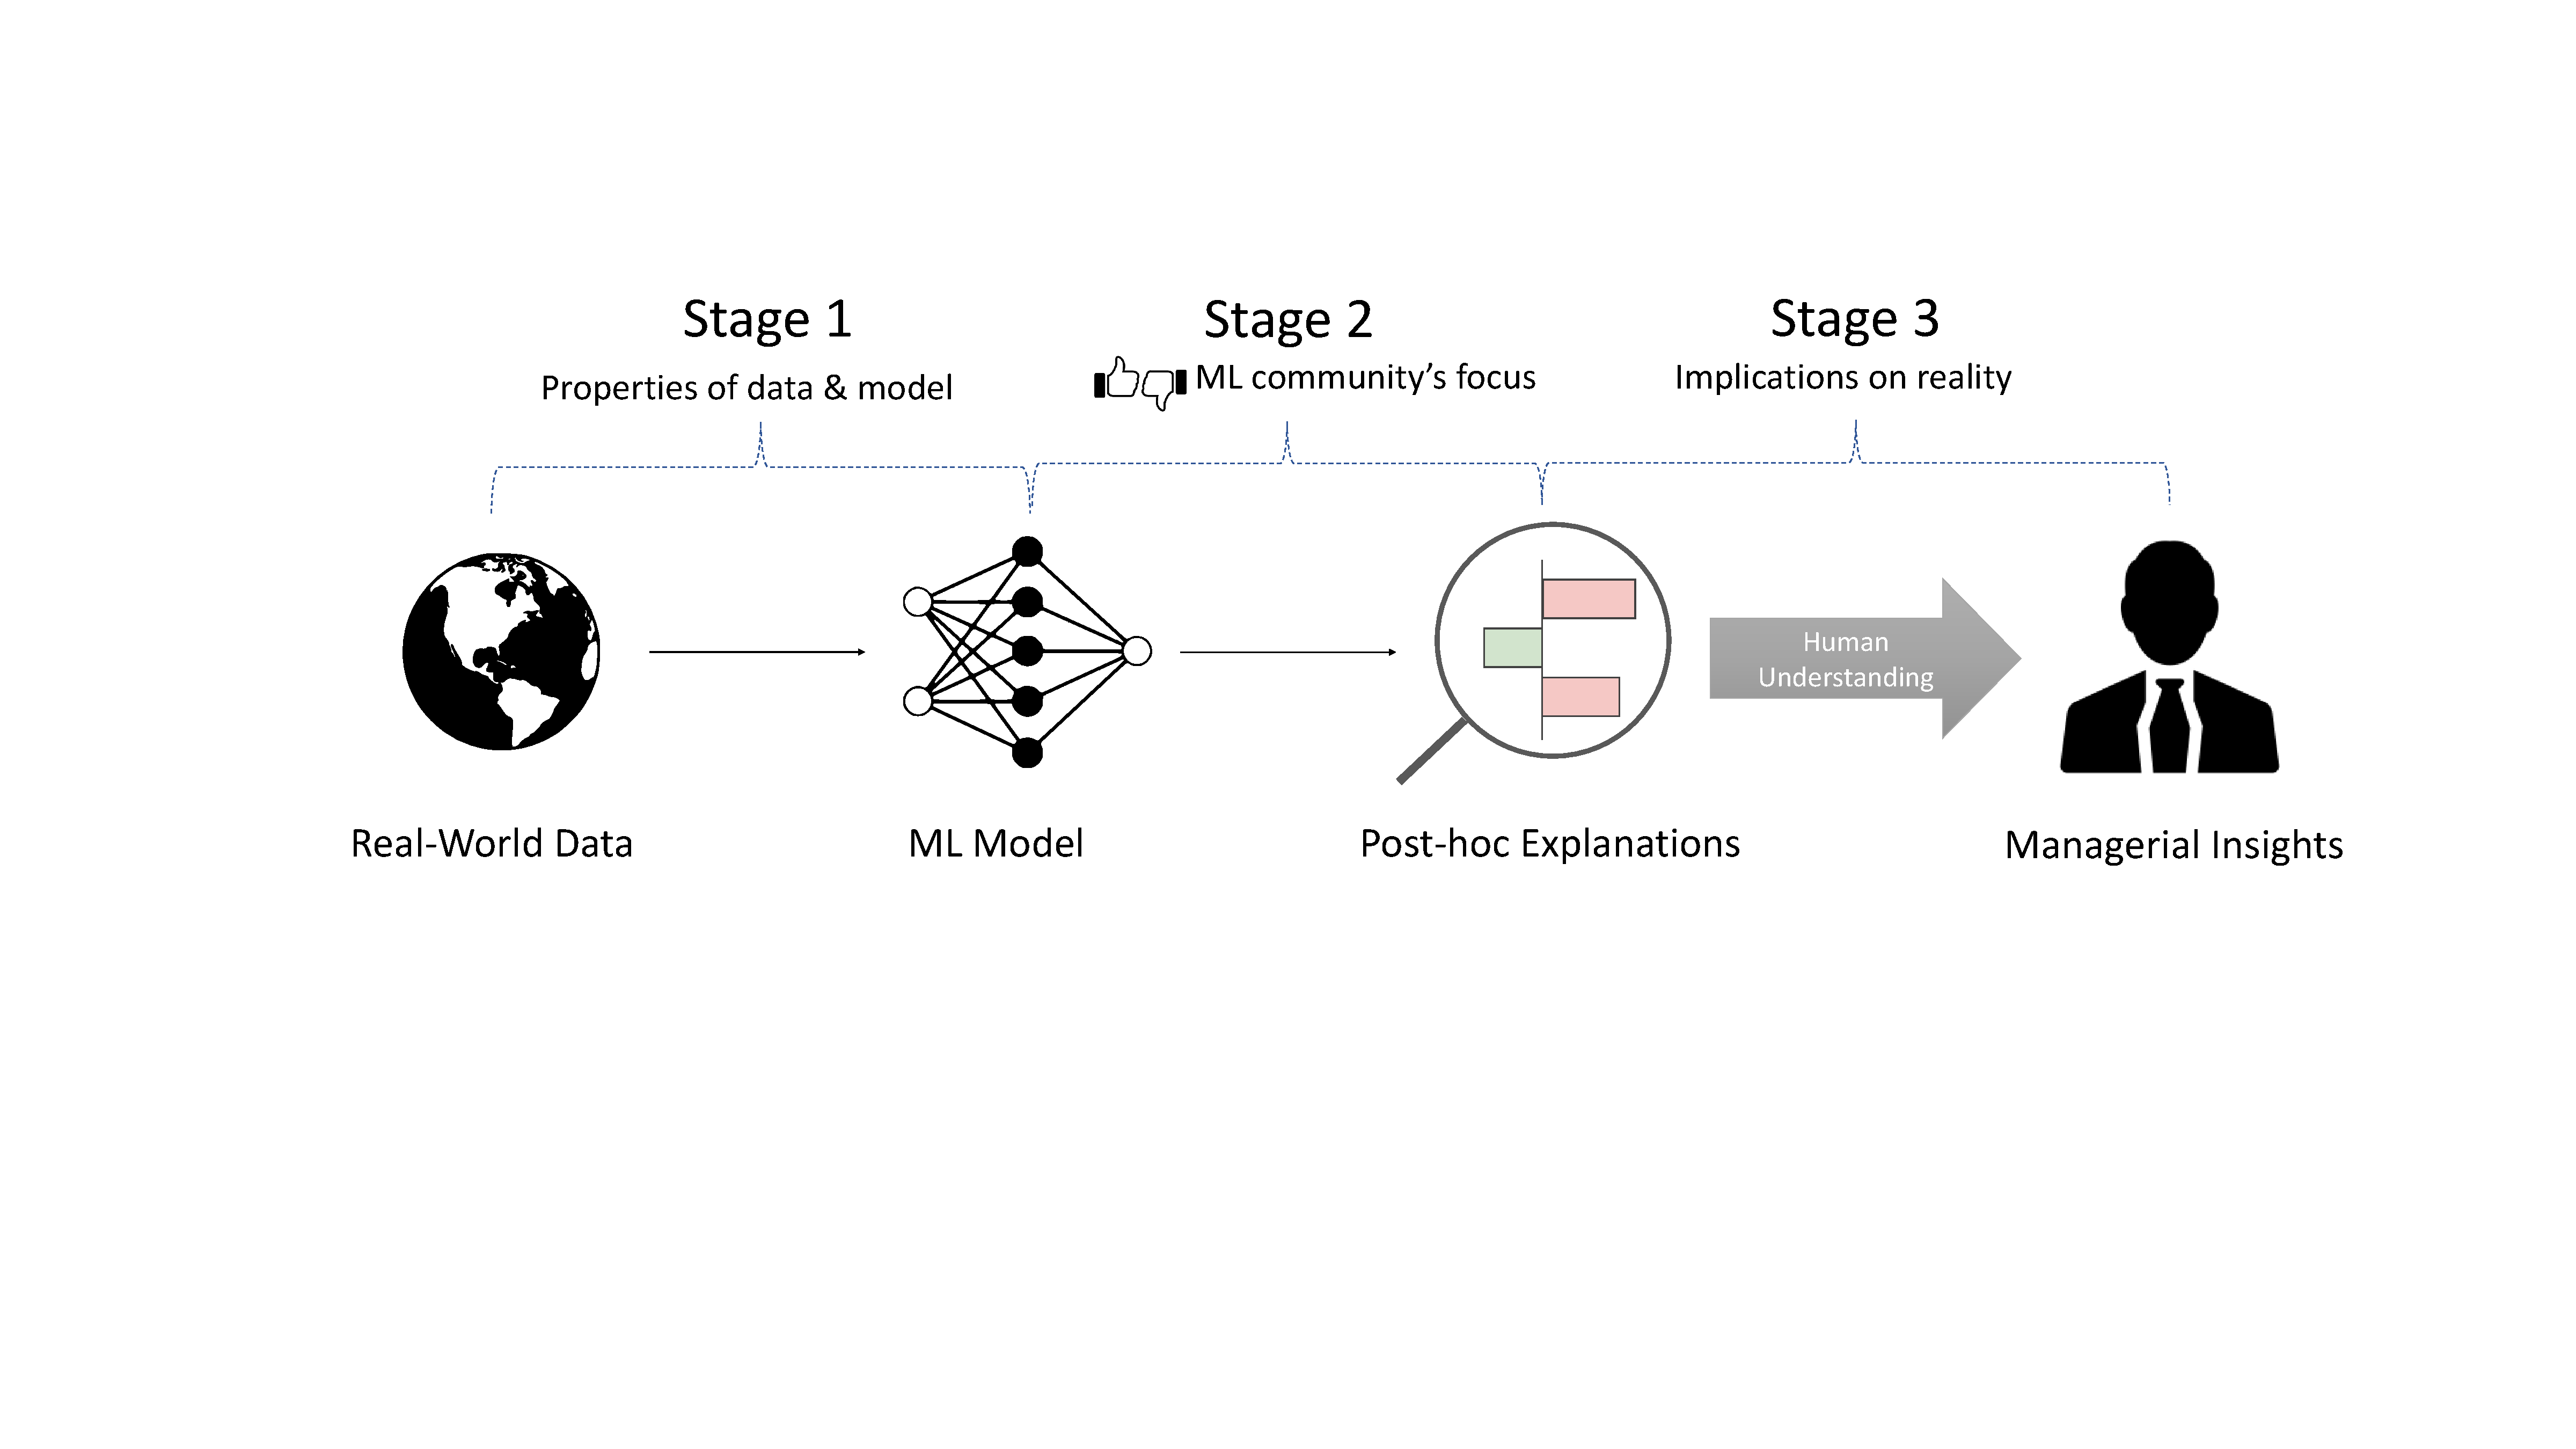
\includegraphics[width = \textwidth,trim=250 500 150 250 mm, clip=true]{Figures/pipeline.pdf}}
        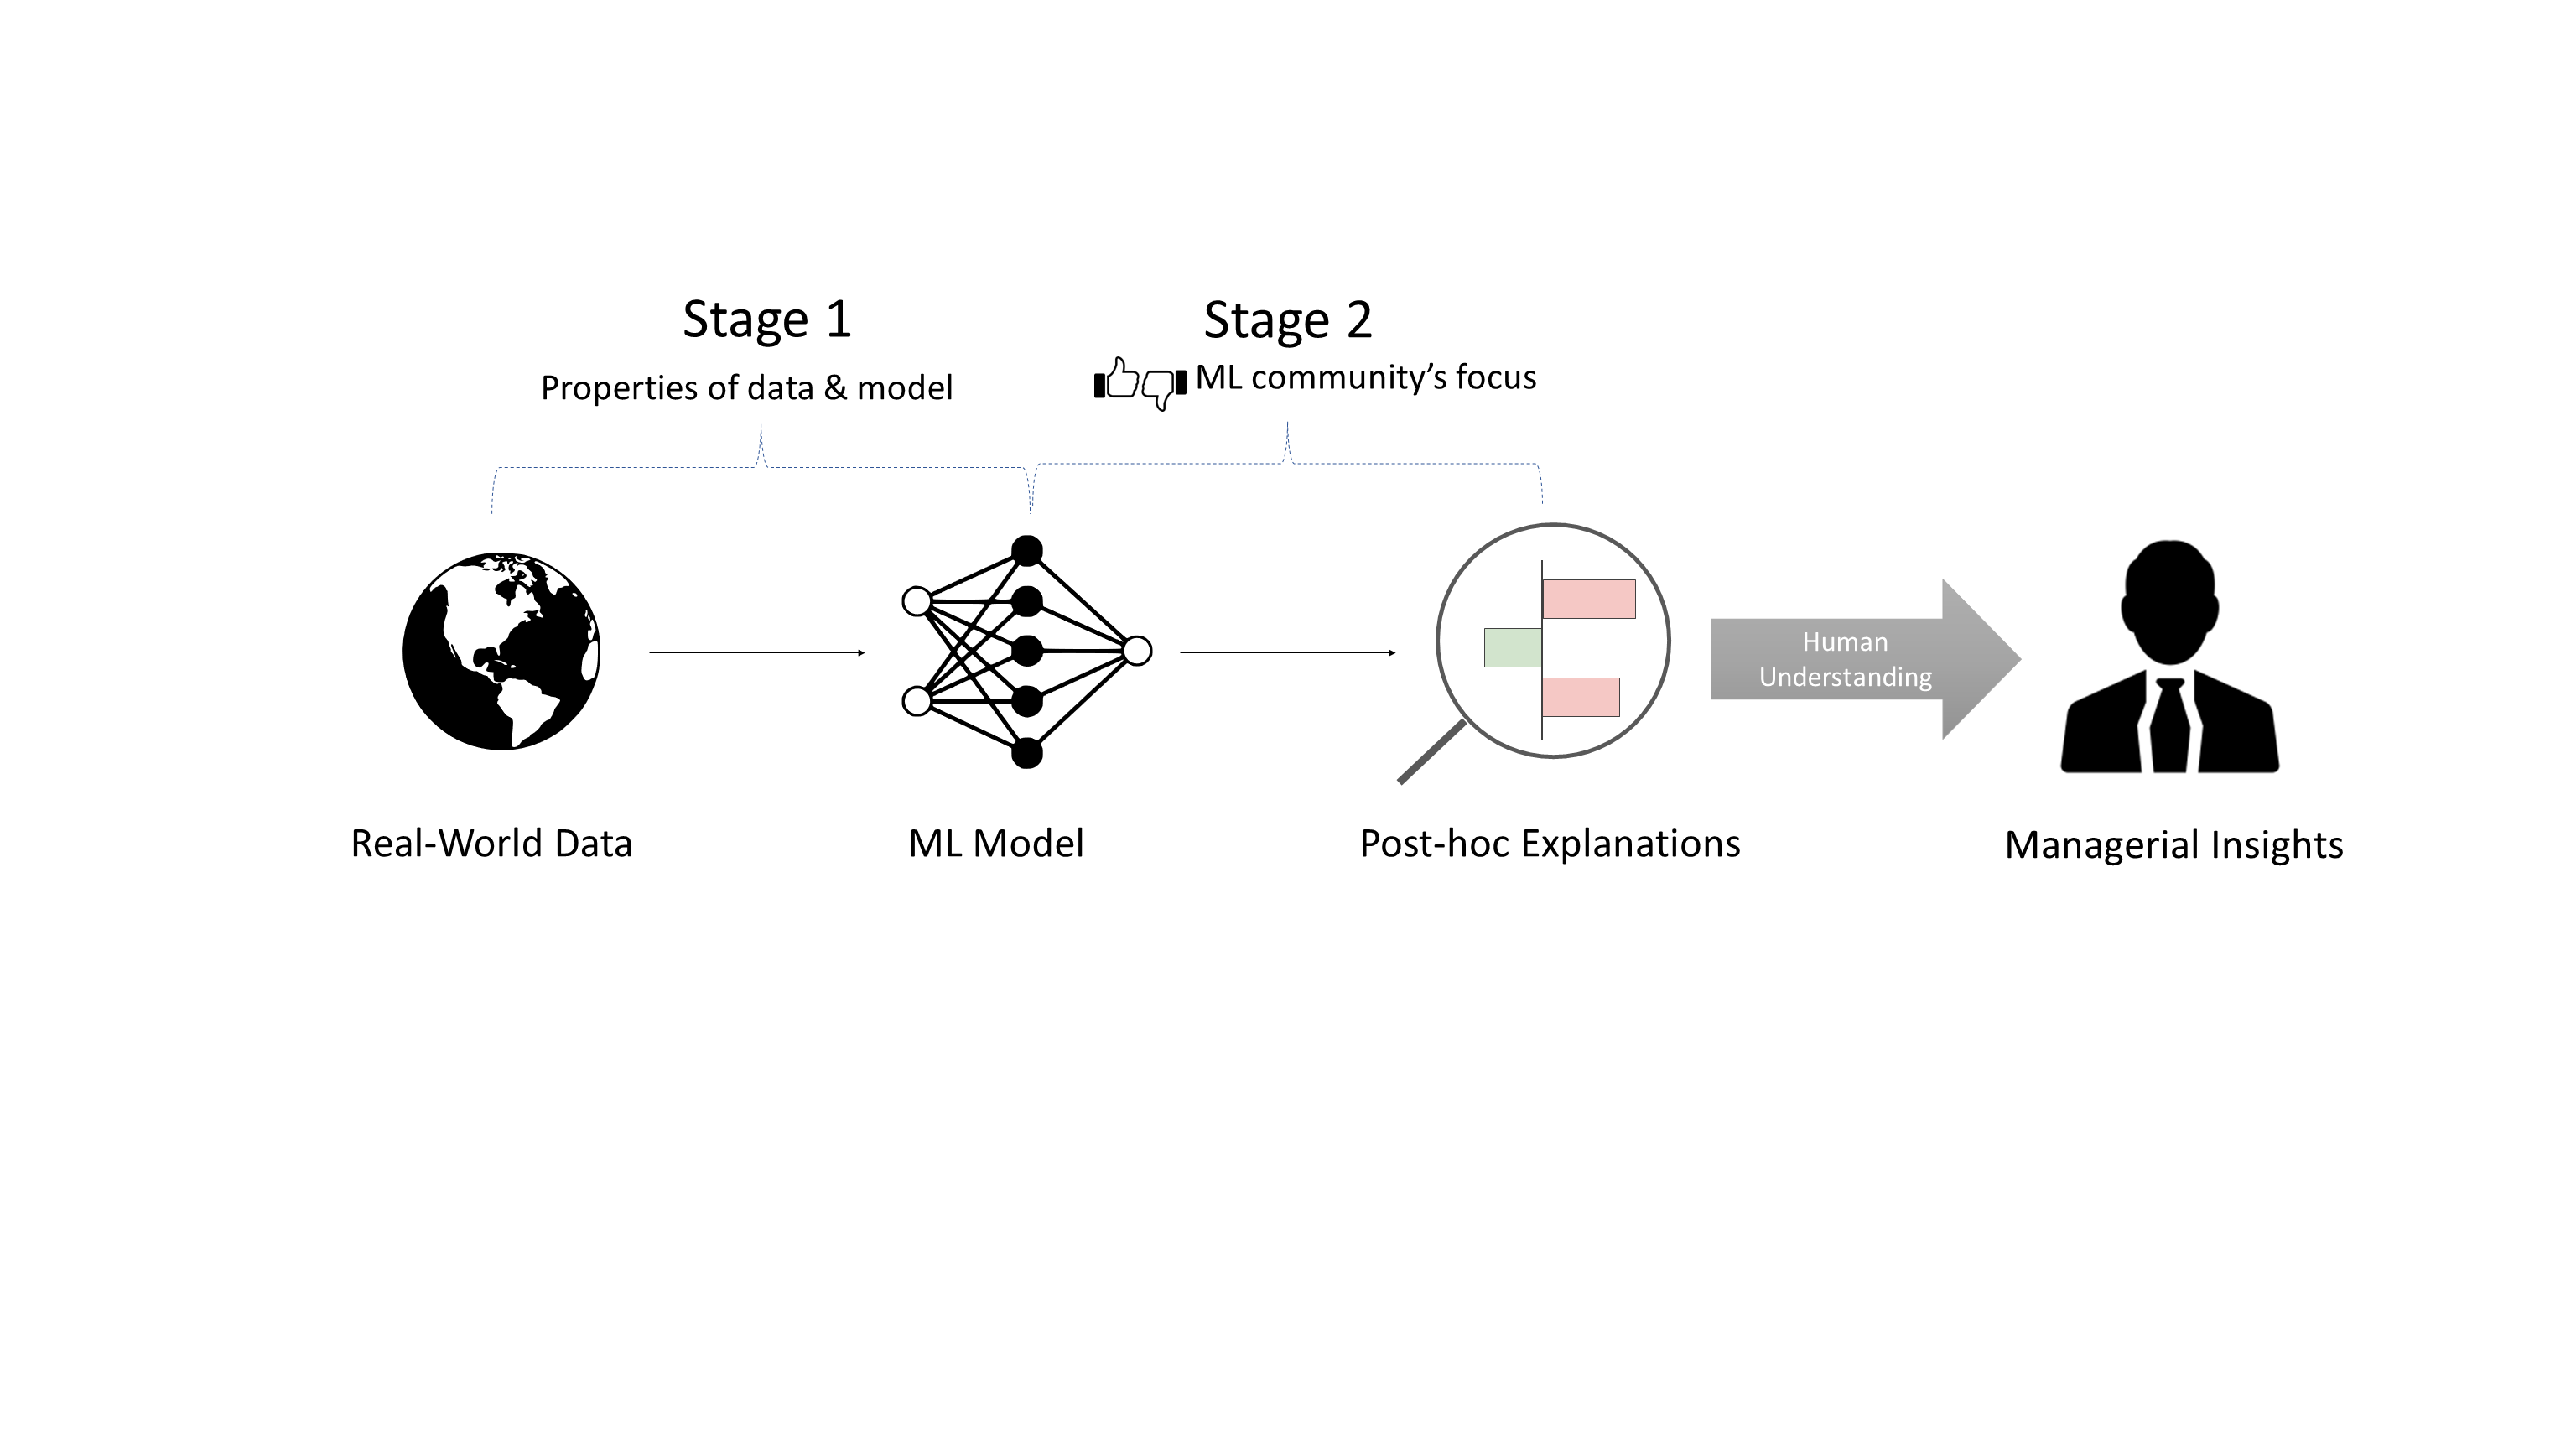
\includegraphics[width = \textwidth,trim=250 500 150 250 mm, clip=true]{Figures/teaser.png}
        \caption{Prediction Insight Pipeline: the pipeline of using post hoc explainers to obtain managerial insights in business research. The ML community has focused on what we call stage 2, explaining a model in isolation.}
        \label{fig:pipeline}
    \end{figure}



Although  LIME and SHAP seem like magical tools which enable interpretability at no cost to predictive accuracy, this paper aims to urge the research community to approach post hoc explanations with skepticism and a more critical eye. An alarm first went off in the machine learning community. In the past few years, machine learning researchers have identified various issues with post hoc explainers, questioning the correctness and validity of explanations \footnote{A review of related work on such issues appears in the next section.}. % We discuss design issues like how different data pre-processing schemes can change what features LIME supposes are important, as well as practical issues like how the form of SHAP explanations are unnatural to humans. This paper is primarily concerned with how post hoc explanations may not be useful to business researchers due to being incorrect and inconsistent.%, or ineffectual when tasked with recommending recourse options. 
However, attention has focused mainly on one leg of the pipeline in Figure \ref{fig:pipeline}, which we call stage 2 of the pipeline. % Machine learning researchers have primarily been concerned with evaluating explanations of black box models instead of  understanding of the data. %without consideration of the mechanism that generated the training data.
This is because the primary goal of the machine learning field is to develop new models that make better or faster predictions. Thus, researchers need to understand the models in order to debug or improve them \citep{lertvittayakumjorn21explanation}, or safeguard against biases \citep{alves21reducing}, etc. On the other hand, the primary goal of business research is to understand the data from which an ML model is trained. In this paper, however, we scrutinize how post hoc explanations can fail to achieve this goal.

LIME and SHAP explanations have been over-generalized in diverse areas of business literature to explain the relationships that exist in the data, such as making inferences about the $\beta$s. This is exemplified by \citet{lorentzen2020peeking}, a tutorial for using LIME and SHAP in actuarial science, which states that post hoc explainers enable ``...the model to serve as a source of information and to validate hypotheses—instead of only serving as a prediction machine". The following are examples where SHAP was used in this manner. \citet{park2024extracting} claimed that SHAP explanations provide guidance on what smartphone features customers prefer. \citet{bali2023option} uses SHAP explanations to claim that the implied volatility of an option is the single most important predictor of its price. Although \citet{kovvuri23fund} uses prior literature and a linear regression to corroborate the values and signs of SHAP feature importances, they go on to use SHAP values as evidence of an answer to an open problem in finance. That is, that only moderate diversification is beneficial to the performance of global equity funds. \citet{zhang2023can} used SHAP explanations to identify features such as whether photos posted online by restaurant reviewers have food in them as important to restaurant survival\footnote{They then use causal forests to try to further understand the treatment effect of those features on restaurant survival.}. Whether or not they happen to be true or justifiable, the validity of these claims entails that the black box models being explained discovered the correct relationships underlying the data and that the explainers faithfully explained the black box models. 

That the meaning of LIME or SHAP feature importance values may not match what researchers desire or expect is another issue. In particular, if estimating $\beta$ is the goal, SHAP is inherently ill-suited for this task. We delve into the technical details of this in Section \ref{sec:theoretical_considerations}. There are many types of feature importance \citep{AchenChristopherH1982Iaur} involving $\beta$. \textcolor{red}{However, none of the works cited in the previous paragraph identified which type they were interested in and justified that the explainer(s) used were actually providing that type of feature importance.} The basic question of why Shapley values are appropriate feature importance measures is never addressed in these works\footnote{It is argued in \citep{kumar20shap} that Shapley values are not conducive for human understanding of feature importance.}. 

% (  Incorrectness is primarily due to approximation. errors from both the explainer and the model being explained, but also due to inconsistency. The most common form of inconsistency is instability, a phenomenon in which an explainer gives very different explanations for similar outcomes, an issue shared by LIME and SHAP~\citep{alvarez18robustness}. LIME can also give different explanations for the same outcome by changing its hyperparameters and random seed~\citep{bansal20sam}. Instability can cause LIME and SHAP to produce inconsistent within themselves, but they can also be inconsistent with each other~\citep{kommiya21towards}.  Researchers also question whether the form of current post hoc explanations are even conducive to human understanding. For exmaple, \cite{kumar20shap} proposes that ``Shapley values are not a natural solution to the human-centric goals of explainability" because, e.g. it is not clear that statistically related features should be considered as separate players in the game-theoretic framework underlying Shapley values. \cite{laugel19issues} states that counterfactual explainers make assumptions about data that make them unreliable, and can result in unrealistic counterfactual examples.) This paper is primarily concerned with how post hoc explanations may not be useful to business researchers due to being incorrect and inconsistent. 

% First, we \textit{theorize} the connection between the $\beta$s from data and the feature importance of LIME and SHAP, respectively, in ideal situations. 


% In summary, this paper makes three main contributions. First, we present the pipeline that existing work often follows to obtain post hoc explanations and show the connection between the $\beta$s from data and the feature importance of LIME and SHAP, respectively, in ideal situations. By doing this, we explain why it is intuitively attempting to use feature importance as a proxy for $\beta$s. Then, we \emph{demonstrate} the issues with post hoc explanations using obtained from the pipeline and \emph{identify} the causes of such issues. Finally, we \emph{test} some simple and intuitive mitigation methods from which we form some recommendations to researchers and practitioners to follow in order to improve the quality of post hoc explanations. 



% To differentiate from prior machine learning works, we evaluate the quality of explanations of a black box model by comparing the explanations with a known ground truth. We address the entire pipeline and pay special attention to stages 1 and 3 in Figure \ref{fig:pipeline}, which has been largely ignored by the machine learning community but is very important to business researchers. That is, we focus on the conditions that cause post hoc explainers to give unfaithful or inconsistent descriptive insights to business researchers, leading to faulty decision making. 









%a company wants to understand customer behavior by analyzing purchase histories or customer feedback. These insights can identify trends in purchasing behavior, such as which products are most popular or which demographics are buying certain products. %Business and managerial insights can be classified into two broad categories, \textbf{descriptive} and \textbf{prescriptive}. Descriptive insights describe what has happened or is happening within a company or market, providing a summary of patterns and trends identified from data. 
%For example, a company might use descriptive insights to understand customer behavior by analyzing purchase histories or customer feedback. These insights can identify trends in purchasing behavior, such as which products are most popular or which demographics are buying certain products.

%On the other hand, prescriptive insights provide recommendations or solutions for future action. Prescriptive insights are generated by analyzing data and building models that help identify the best course of action. These insights help businesses optimize their operations, improve their customer experience, or increase revenue. For example, a company might use prescriptive insights to optimize its supply chain by analyzing data on inventory levels, shipping times, and supplier performance. Based on this analysis, the company could identify opportunities to improve efficiency, reduce costs, and improve customer satisfaction.
%Overall, descriptive insights provide a snapshot of the past and present, while prescriptive insights offer recommendations for the future. Both types of insights are valuable for businesses and can drive better decision-making and improve overall performance.

% The two central goals of this paper are to alert business researchers to issues with post hoc explainers that are of particular importance to the business research community and to propose and test some mitigation strategies for the issues we identify.  

% \textbf{Feature Importance and $\beta$s}


% \textbf{Issues with Post hoc Explanations}
We identify two classes of issues with post hoc explainers that inhibit $\beta$ estimation, \textit{unfaithfulness} and \textit{inconsistency}. Unfaithfulness refers to post hoc explanations deviating from the truths underlying the data and inconsistency refers to explanation disagreement among themselves. Evaluating the quality of explanations requires the ground truth explanation from the data. However, we do not directly compare LIME and SHAP explanations against $\beta$s since their importance measures and $\beta$s, while correlated, are obtained in a different way and the actual values are not directly comparable. Therefore, we compare the second order of the two types of results. The first evaluation is the sign of feature importance. Compared against the true sign from $\beta$, this evaluation measures whether the post hoc explanations can correctly reflect the qualitative relationship between an independent variable and the target variable. The next evaluation is on the ranking of features using the feature importance values, compared against the ranking using $\beta$. This evaluation measures the relative importance of each feature. Since practical attribution analysis often focuses more on the most important features, we also use a recall metric, which in our context measures the correct identification of the top $K$ features. 


%measured against the ground truth from data. Here we use a loser definition of  ``ground truth'', which is as the second order results from the actual values of $\beta$.  %We expect faithful explanations to assert that features are comparatively more and less important in the same ways they are in reality. %For a minimal sales example, suppose that promotions have a strong positive effect on sales and discounts do not affect sales, but a LIME explanation of a purchase of an item which was promoted and on sale gives a large positive feature importance value to the sale and a small positive importance value to the promotion. A faithful explanation would have given the sale feature no importance (or at least less importance than discounts). 
% In the aforementioned loan application scenario, if we suppose that having a cosigner is more important than low credit utilization, post hoc explanations of application decisions should convey this information.
%Meanwhile, inconsistency occurs when a collection of explanations do not, together, tell a consistent narrative. A common symptom of inconsistency is seen when different explanations are obtained for the same input. Fixing one input, a post hoc explanation of that input is influenced by the dataset it comes from, the black box being explained, and the explainer itself. Returning to the loan application scenario, inconsistency can manifest if, for example, an explainer implies that credit score is the most important feature for one applicant and income is the most important feature for another. %In the previous hypothetical marketing problem, LIME could give the most importance to promotions, while SHAP could give the most importance to sales when explaining the same purchasing event.  %The primary issue is incorrectness. This could cause business researchers trying to understand FICO credit scores to, say, incorrectly think FICO weighs credit inquiries more than delinquent payments. Secondarily, we study inconsistency. This could cause two researchers in the same lab studying the same model and credit score data to obtain totally different views of how credit scores work. 

    We design various experiments to demonstrate consequences of unfaithful and inconsistent explanations that appear even when the ground truth is a linear model. We find that in rather simple simulated business scenarios with a linear ground truth model, LIME and SHAP explanations often fail to reproduce the insights we intend them to find. Their explanations are even imperfect under ideal conditions where the black box being explained is highly accurate, capable of capturing the causal relations underlying its training data, and the training data's features are all observed, mutually independent, and unconfounded (these will be discussed in more detail in Section \ref{sec:data_related_issues}) in addition to the typical i.i.d. assumption necessary for machine learning. The evidence we present for LIME and SHAP's failures in explaining linear models should make researchers very cautious in using LIME or SHAP to explain general non-linear phenomena.%black box functions.
    
    This being the case, we provide theoretical results on the respective abilities of LIME and SHAP to capture $\beta$ and use those results to propose and test some intuitive mitigation strategies meant to aid $\beta$ estimation. In particular, we found evidence that averaging explanations of a family of accurate models both increases explanation quality and addresses the problem of choosing which black box to explain. We also found that ensuring that the training data used by the black box being explained satisfy causal inference conditions is associated with increasing the faithfulness of explainers. However, other intuitive strategies, such as averaging explanations of a single black box between two given by LIME and SHAP were ineffective. Our proposed mitigations do not completely solve unfaithfulness and inconsistency; LIME and SHAP remain tools that business researchers must use with caution. %add something about robustness/causal forest here??????

    
    %Explainable ML  methods are wrappers around black-box ML models used for explanations of the black-boxes. In addition to university research groups using post hoc explanations to explain black-box models for loan approval prediction~\citep{dumitrache19loan approval}, financial risk~\citep{yang21financial}, and e-commerce reviews~\citep{meng21online_review}, large companies like Microsoft~\citep{mothilal20dice} and Uber~\citep{chen20causalml} have developed their own software and methods for XML.

    % Unfortunately, issues abound with using post hoc explanations to draw such managerial insights. The machine learning community is the first to criticize post hoc explainers \citep{rudin18stop} and has pointed out both theoretical and practical issues with using post hoc explainers to explain a black-box \citep{ add a few representative papers or review papers}. A main complaint is that post hoc explanations are often not faithful to the original black-box model and do not represent what really happens in the decision-making processes. post hoc explainers are thus even discouraged in favor of usage of intrinsically interpretable ML models for these reasons~\citep{rudin18stop}. %As will be shown in Section \ref{sec:related_work} there is a slew of publications from the computer science literature pointing out both theoretical and practical problems with XML methods. 
    % However, papers from the machine learning community stop at the stage of explaining the model since the machine learning community is mainly concerned with the model performance. The business community, on the other hand, uses the post hoc explainer for the purpose of obtaining understanding of the data and underlying phenomenon, and new issues arise with post hoc explainers in this aspect. Therefore, in this paper, we specifically focus on the context of  using post hoc explanations in business research to obtain ``insights'' about the data.
    
    % We represent the pipelines that most business research follows when they use post hoc explanation with a two stage framework.   In the first stage, a post hoc explainer is used to interpret the outputs of a black-box model. In the second stage, information gleaned from explanations of the black box model is used to draw managerial insights about the business process described by the input data. We treat issues in the first and second stages separately and give guidelines for them separately, but anything applicable to stage 1 is also applicable to stage 2.
    % This pipeline is shown in Figure \ref{fig:teaser}. 
    

    % The machine learning researchers only use post hoc explanations for stage 1: their goal is only to explain the black-box model, but the business researchers use the post hoc explanations to obtain insights for underlying real-world phenomena, which includes both stage 1 and stage 2 in the above pipeline.  Thus, there are unique issues with post hoc explanations that have not been systematically studied or even identified for this purpose.


   
   
     % In this paper, though, we assume that either the business problems of interest are of low-stakes or development of an intrinsically interpretable model is infeasible or leads to unsatisfactory results. Following the Rashomon Set theory~\citep{semenova22rashomon}, there are cases where it may be infeasible to find an intrinsically interpretable model with sufficiently good performance. As such, the best remaining option would be to explain a black-box model that does have good enough performance. 


%Two types of managerial insights we usually need in business research. 1) Which feature(s) is (are) important for the current outcome? For example, which feature is important for customer loan approval, sales, loan application approval? 2) Which feature(s) can be changed to get a different outcome? For example, if a customer's loan application failed, what do we recommend the customer to do to get it approved? If the sales are bad, what should we do to increase the sales.

%Researchers sometimes use black-box models and then rely on post hoc explanations to get explanations or insights that answer the two types of questions above. However, ........ So the goal of this paper is to identify the issues arise in the process of generating explanations and using explanations to get the managerial insights. We then recommend a list of procedures users need to do in order to improve the success/correcteness of the explanations.

   Our main contributions can be grouped into the following two parts. First, we give a novel systemization of the use of post hoc explainers that illuminates how and why post hoc explainers may not give business researchers faithful managerial insights, as well as what kinds of errors the explanations can contain and how the errors could negatively affect businesses and researchers. Our proposed system addresses vulnerabilities in the pipeline shown in Figure \ref{fig:pipeline} that business researchers are encouraged to keep in mind or mitigate in order to successfully glean managerial insights from post hoc explainers. We develop the system over the course of the paper by first demonstrating the issues, then identifying the causes of the issues. The second main component of our contributions is a set of mitigation strategies for unfaithfulness and inconsistency that we propose and test. Many papers in the machine learning literature have explored the weaknesses of post hoc explainers, but to the best of our knowledge, no other work has discussed how the issues with post hoc explainers could yield unfaithful managerial insights.   %Second, we provide guidelines to help avoid being misled by incorrect post hoc explanations. 

Our system addresses the following questions which are of particular interest to the business community, and therefore not investigated in prior machine learning works on post hoc explainer efficacy. 
\begin{enumerate}
    \item How well can post hoc explanations faithfully explain a simple linear ground truth underlying a black box model's training data?
    \item Will explanations obtained from different configurations of the pipeline contain an internally consistent narrative, such that I do not need to worry too much about my choice of data preprocessing, black box, explainer, and explainer settings? 
    \item What strategies can I adopt to increase the likelihood that the managerial insights I glean from post hoc explanations are actually valid in reality?
    %\item What steps can I take to address choice paralysis induced by the many possible configurations of the pipeline?
\end{enumerate}

    The paper is organized as follows. We will review related work in Section \ref{sec:related_work}. Then we will use a simulated data set with ground truth models that we create to demonstrate the \pipeline and its vulnerabilities. We then discuss the potential issues with post hoc explanations that arise at different stages of the pipeline to lead to unfaithful descriptive insights. Question 1 is treated in Section \ref{sec:unfaithfulness}. Question 2 is treated in Section \ref{sec:inconsistency}. Having demonstrated the issues via experiments, we explore how they may be addressed using theoretical results presented in Section \ref{sec:theoretical_considerations}. Proofs appear in the Appendix. In Section \ref{sec:incorrectness_mitigation} we provide mitigation strategies for unfaithfulness and in Section \ref{sec:inconsistency_mitigation} we provide mitigation strategies for inconsistency. We propose a general strategy based off of our best mitigations to explore in Section \ref{sec:summary_and_strategies}. We test it in Section \ref{sec:case_study} by gauging how beneficial it is over a baseline in reproducing the findings of an econometrics study done on real loan data. The paper concludes in Section \ref{sec:discussion} with a summary of our findings.
    
\section{Related Work}
    \label{sec:related_work}
    \begin{itemize}
    
    \item This section introduces popular post hoc explainers and then reviews the prior literature discussing their weaknesses. 
    

    %\subsection{Background on LIME and SHAP}
     \item LIME and SHAP are model-agnostic attributive post hoc explainers. 
        
    \item Both LIME and SHAP represent feature importance values with the coefficients of an additive surrogate model.
    
    %\subsubsection{Inconsistency}
    \item One key issue that make LIME and SHAP difficult to trust is that they are prone to giving different, possibly conflicting, explanations for the same input. 
    
    \item The choice of which black box to explain is an additional source of inconsistency.
        
    \item Another form of inconsistency called instability occurs when an explainer gives drastically different explanations for similar inputs to the model being explained \citep{molnar2019}. 
    
    \item The accuracy (or fidelity) of an explainer is another multifaceted issue with many consequences. LIME has been proven to always have some approximation error with respect to the black box it is explaining that can lead to unfaithful explanations; \cite{garreau20theoretical} showed that LIME's surrogate model generally has non-zero local error. 

    \item However, generally speaking, an explanation of a black box machine learning model should not be expected to allocate importance to features in this way. 

    \item For a post hoc explainer to give causal insights about reality by explaining a black box model trained on i.i.d. observational data, the data must satisfy conditions for causal inference.
    \end{itemize}

\section{Prediction Insight Pipeline}
    \label{sec:pipeline_demo}
    In this section, we will define each step of the pipeline and demonstrate it using simulated loan approval data, variants of which will be used throughout the paper. 

 \subsection{Generating Simulated Data}
    \begin{itemize}
 \item We construct a total of ten features, where four are demographic features including age, sex, marital status and income, and the other six are credit-related features including, the number of credit inquiries in the past year, whether the applicant has a loan cosigner, the credit utilization rate, the number of delienquent payments, the credit score, and an unobserved measure of social support which is only used by the ground truth model but not available to machine learning models.


\begin{table}[h]
\centering
\resizebox{\textwidth}{!}{%
\begin{tabular}{c|cccc}
%\toprule
\hline
\textsc{Feature} & \textsc{Explanation}                           & \tetextscxtbf{Formula}       & \textsc{Input to $\mathcal{G}$} & \textsc{Input to $\mathcal{M}$}                            \\ \hline%\Xhline{0.5ex}%\toprule
%\rowcolor[gray]{.9}
Age              & Applicant Age                                   & Uniform(18,100)        &  \checkmark & \checkmark                                            \\ 
%\rowcolor[gray]{.9}
Sex              & Applicant Sex                                   & Bernoulli(.5)          &  \checkmark & \checkmark                                              \\
Married          & Applicant Marital Status                        & Bernoulli(.5)          &  \checkmark & \checkmark                                              \\ 
Income           & Applicant Income                                & Normal(40,000, 30,000) & \checkmark & \checkmark  
\\ 
Inquiries         & Number of credit inquiries                     & Uniform(0,6)           &  \checkmark & \checkmark                                              \\ 
Social Support   & \makecell{0 = no support\\ 1 = perfectly supported}        & Uniform(0,1)           & \checkmark &                                  \\ 
Cosigner         & \makecell{Indicator of presence \\of loan cosigner}         & Bernoulli(.5)          & \checkmark & \checkmark   \\ 
%Economy          & Health of the economy in the customer's region & Uniform(0,1)           &                                %              \\ \hline

%\rowcolor[gray]{.9}
Utilization      & \makecell{Proportion of total \\credit utilized}            & Uniform(0,1)           & \checkmark & \checkmark  
\\ 
Delinquencies    & \makecell{Number of delinquent \\ payments in last 2 years}                   & Uniform(0,24)          &  \checkmark & \checkmark                                             \\ 
%\rowcolor[gray]{.9}

%\rowcolor[gray]{.9}
Credit Score     & \makecell{Credit score based\\ on FICO scoring}             & FICO credit scoring model  \citep{ligons_fico}            & \checkmark & \checkmark                                              \\ \hline%\bottomrule
\end{tabular}%
}
\caption{Description of features for simulated loan data.}
\label{tab:simulated}
\end{table}


   \item Then we define a ground truth model $\mathcal{G}$ for generating the labels, approved, or rejected.
   
    \item We define $\mathcal{G}$ as a multinomial logit model taking standardized features as input\footnote{Note that for this demonstration we use all the features except for social support and will investigate how the data affects explanations later in the paper by changing what features we use.} 
    
   \item  Below, we apply the Prediction Insight Pipeline to a dataset of 5000 simulated application results to demonstrate how one obtains understanding of the data via post hoc explanations.
    \end{itemize}

\subsection{Applying the Prediction Insight Pipeline}
\label{sec:applying_to_simulated}
\begin{itemize}
\item The Prediction Insight Pipeline consists of two stages, building an ML model and explaining the model.

\item To start the pipeline, we train a model, denoted by $\mathcal{M}$, on our simulated data set. 

\item We will demonstrate the pipeline using post hoc explanations for an applicant we will call John.

    \begin{figure}[ht!]
        \centering
            \begin{subfigure}[t]{.48\textwidth}
              \centering
              %\includegraphics[height=.5\linewidth]{Figures/lime_ex_feat.png}%}%{Figures/feng_fig/acc_increase_iter_2.png}
                \begin{tabular}[b]{l|l}
                \toprule
                \textbf{Feature} & \textbf{Value} \\ \hline
                Inquiries        & 0              \\
                Income           & \$38,000       \\
                Delinquency      & 2              \\
                Married          & Yes            \\
                Credit Score     & 760            \\
                Credit History   & 30 months      \\
                Utilization      & 19\%           \\
                Cosigner         & Yes            \\
                Age              & 43             \\
                Sex              & Male   \\   \bottomrule
                \end{tabular}
              \caption{John's feature values}
              \label{fig:lime_ex_feat}
            \end{subfigure}%
            \hfill
            \begin{subfigure}[t]{.48\textwidth}
              \centering
              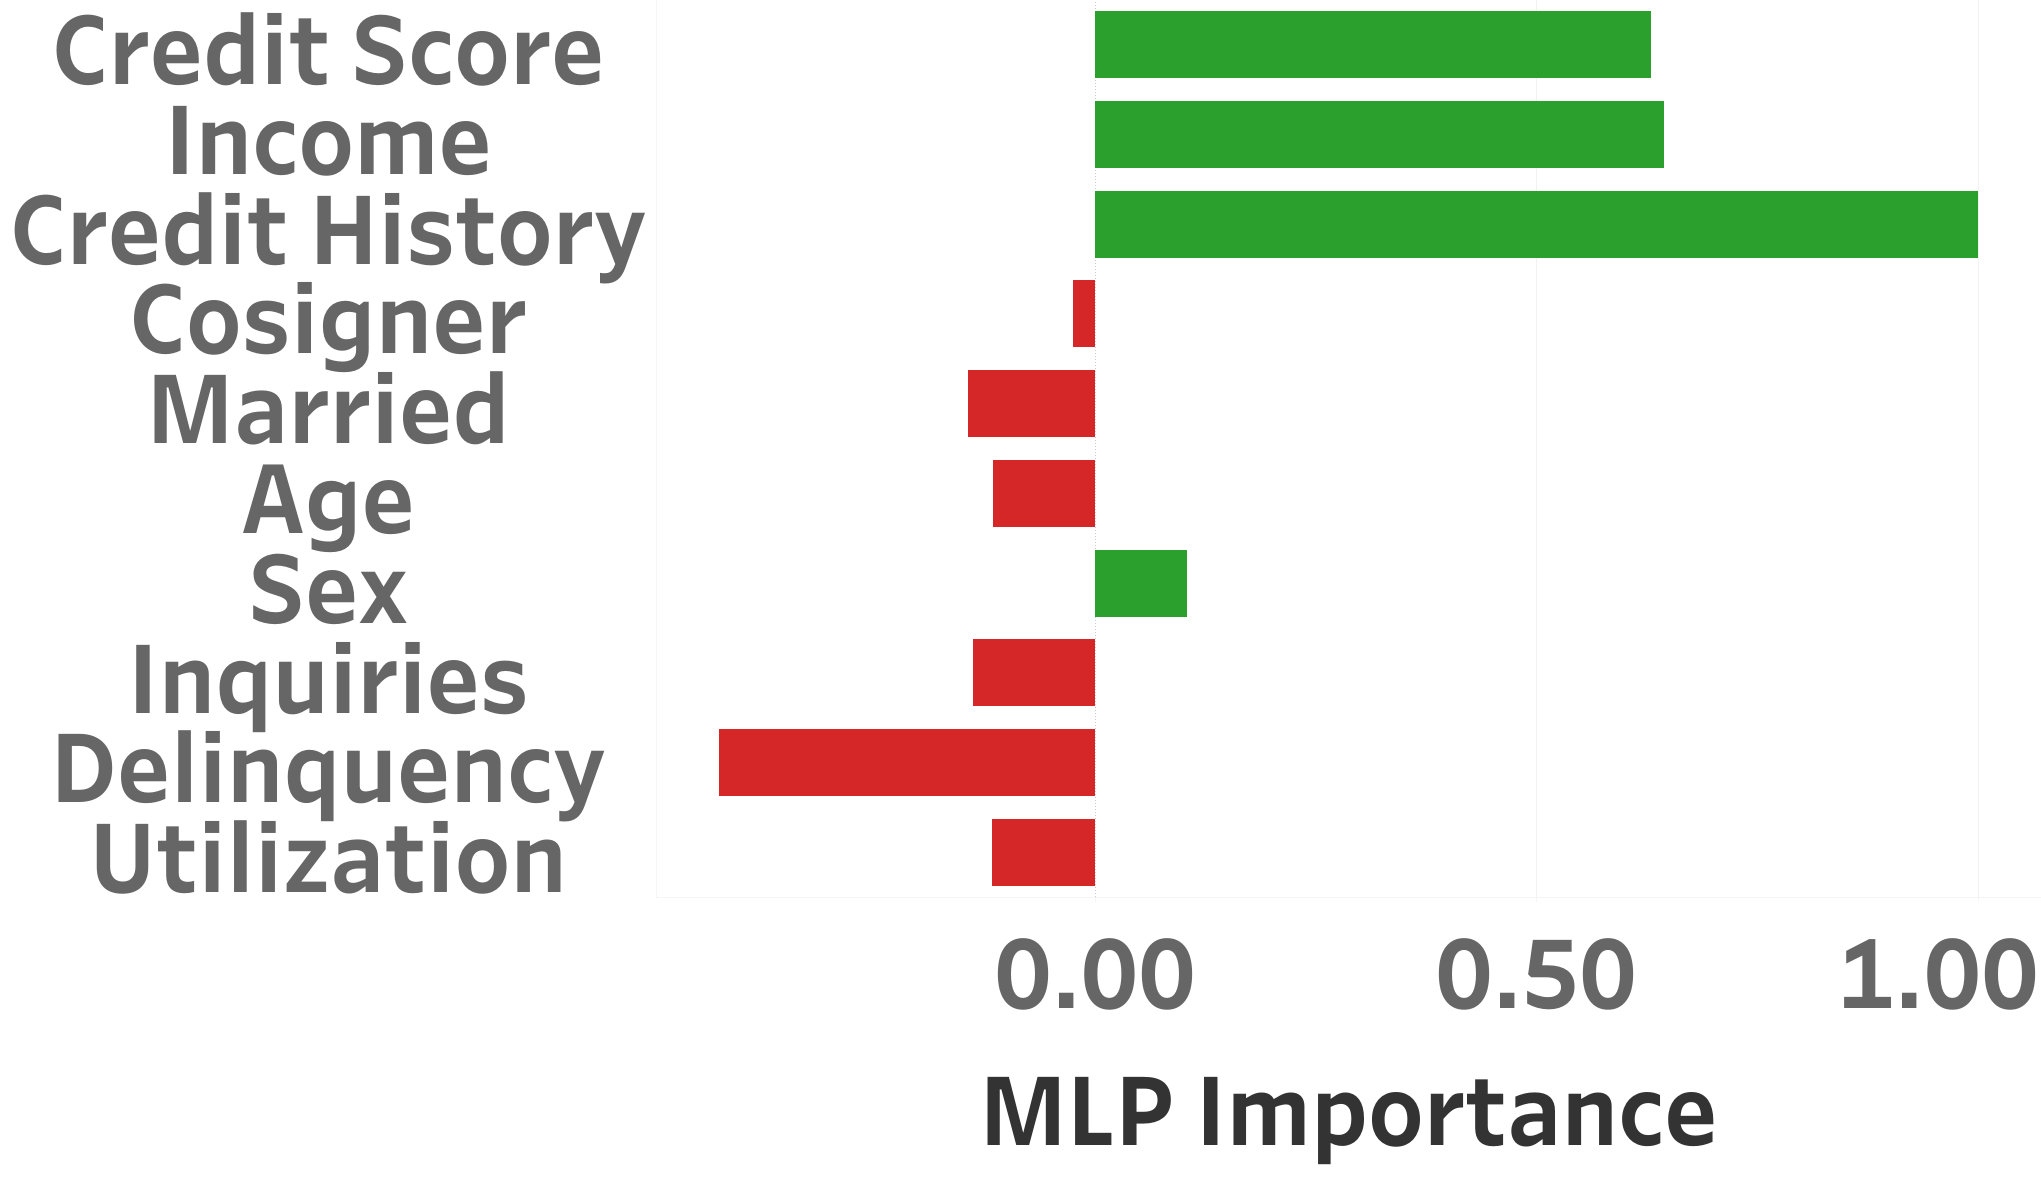
\includegraphics[width=\linewidth]{Figures/lime_ex.png}%}%{Figures/feng_fig/acc_increase_size_2.png}
              \caption{John's explanation}
              \label{fig:lime_ex}
            \end{subfigure}
        \caption{John's demographics along with the output of the LIME package for why John's loan application was approved based on those demographics. The left side of (b) indicates $\mathcal{M}$'s probabilities for each class, and the right side of (b) quantifies the extents to which LIME says each feature is important to each class. The numbers correspond to the LIME surrogate model coefficients $\beta^{\text{LIME}}$. Features listed on left side (for approval $=$ No), have negative coefficients in $\beta^{\text{LIME}}$.}
        \label{fig:lime_ex_full}
        \end{figure}

\item The prediction probabilities on the left side tell us that $\mathcal{M}$ predicted that the individual would be accepted with probability $0.88$. 

\item In the final stage of the pipeline, we inspect the LIME coefficients to try to understand the decision of $\mathcal{G}$.
\end{itemize}
\subsubsection{Unfaithfulness Within a Pipeline and Inconsistency Across Pipelines}
\begin{itemize}
   \item We see from the difference in relative magnitudes of the coefficients from $\beta^{\text{LIME}}$ in Figure \ref{fig:lime_ex} and the ground truth in Equation \ref{eqn:gt} that the explanation for John's approval is unfaithful. 
   
%\subsection{Inconsistency Across Pipelines}
    \item Figure \ref{box} shows results of our simulations for the two researchers. We compare the LIME explanations they receive with the ground truth.
     
\settowidth\mylenC{\textbf{$\mathcal{M}=\text{\textbf{XGBoost}}$}} 
% determine usable width of cols 2 and 3:
\setlength\mylenD{(.3\linewidth-3\tabcolsep)/3}

%  Extra newlien at top necessary so far due to outdated packages
\begin{tcolorbox}[tabular = {*{9}{wc{\mylenD}}}, hbox,center,label = {pipelines_3_ex}]
\\%\midrule
\noalign{\vspace{-\normalbaselineskip}}
%\multicolumn{2}{c}{} & \multicolumn{2}{c}{$\mathcal{E}=\text{\textbf{LIME}}$}  & \multicolumn{2}{c}{$\mathcal{E}=\text{\textbf{LIME}}$} \tabularnewline \midrule
\multicolumn{3}{c}{\textsc{$\mathcal{G}$}} & \multicolumn{3}{c}{\textsc{Pipeline 1: }$\mathcal{M}=\text{\textsc{MLP}}$}  & \multicolumn{3}{c}{\textsc{Pipeline 2: }$\mathcal{M}=\text{\textsc{XGBoost}}$} \tabularnewline \cmidrule(lr){1-3}\cmidrule(lr){4-6}\cmidrule(lr){7-9}%\midrule
\multicolumn{3}{c}{\textsc{Ground Truth}} &\multicolumn{1}{wc{\mylenD}}{$\mathcal{E}$} & \multicolumn{1}{wc{\mylenD}}{\textsc{Accuracy}} & \multicolumn{1}{c}{\textsc{AUC}} & \multicolumn{1}{wc{\mylenD}}{$\mathcal{E}$} &\multicolumn{1}{wc{\mylenD}}{\textsc{Accuracy}} & \multicolumn{1}{wc{\mylenD}}{\textsc{AUC}}\tabularnewline\midrule
 & & & \multicolumn{1}{wc{\mylenD}}{LIME} &\multicolumn{1}{wc{\mylenD}}{.85} & \multicolumn{1}{wc{\mylenD}}{.95} & \multicolumn{1}{wc{\mylenD}}{LIME} &\multicolumn{1}{wc{\mylenD}}{.85} & \multicolumn{1}{wc{\mylenD}}{.92}\tabularnewline %\midrule
\multicolumn{3}{c|}{\begin{minipage}{.3\textwidth}
      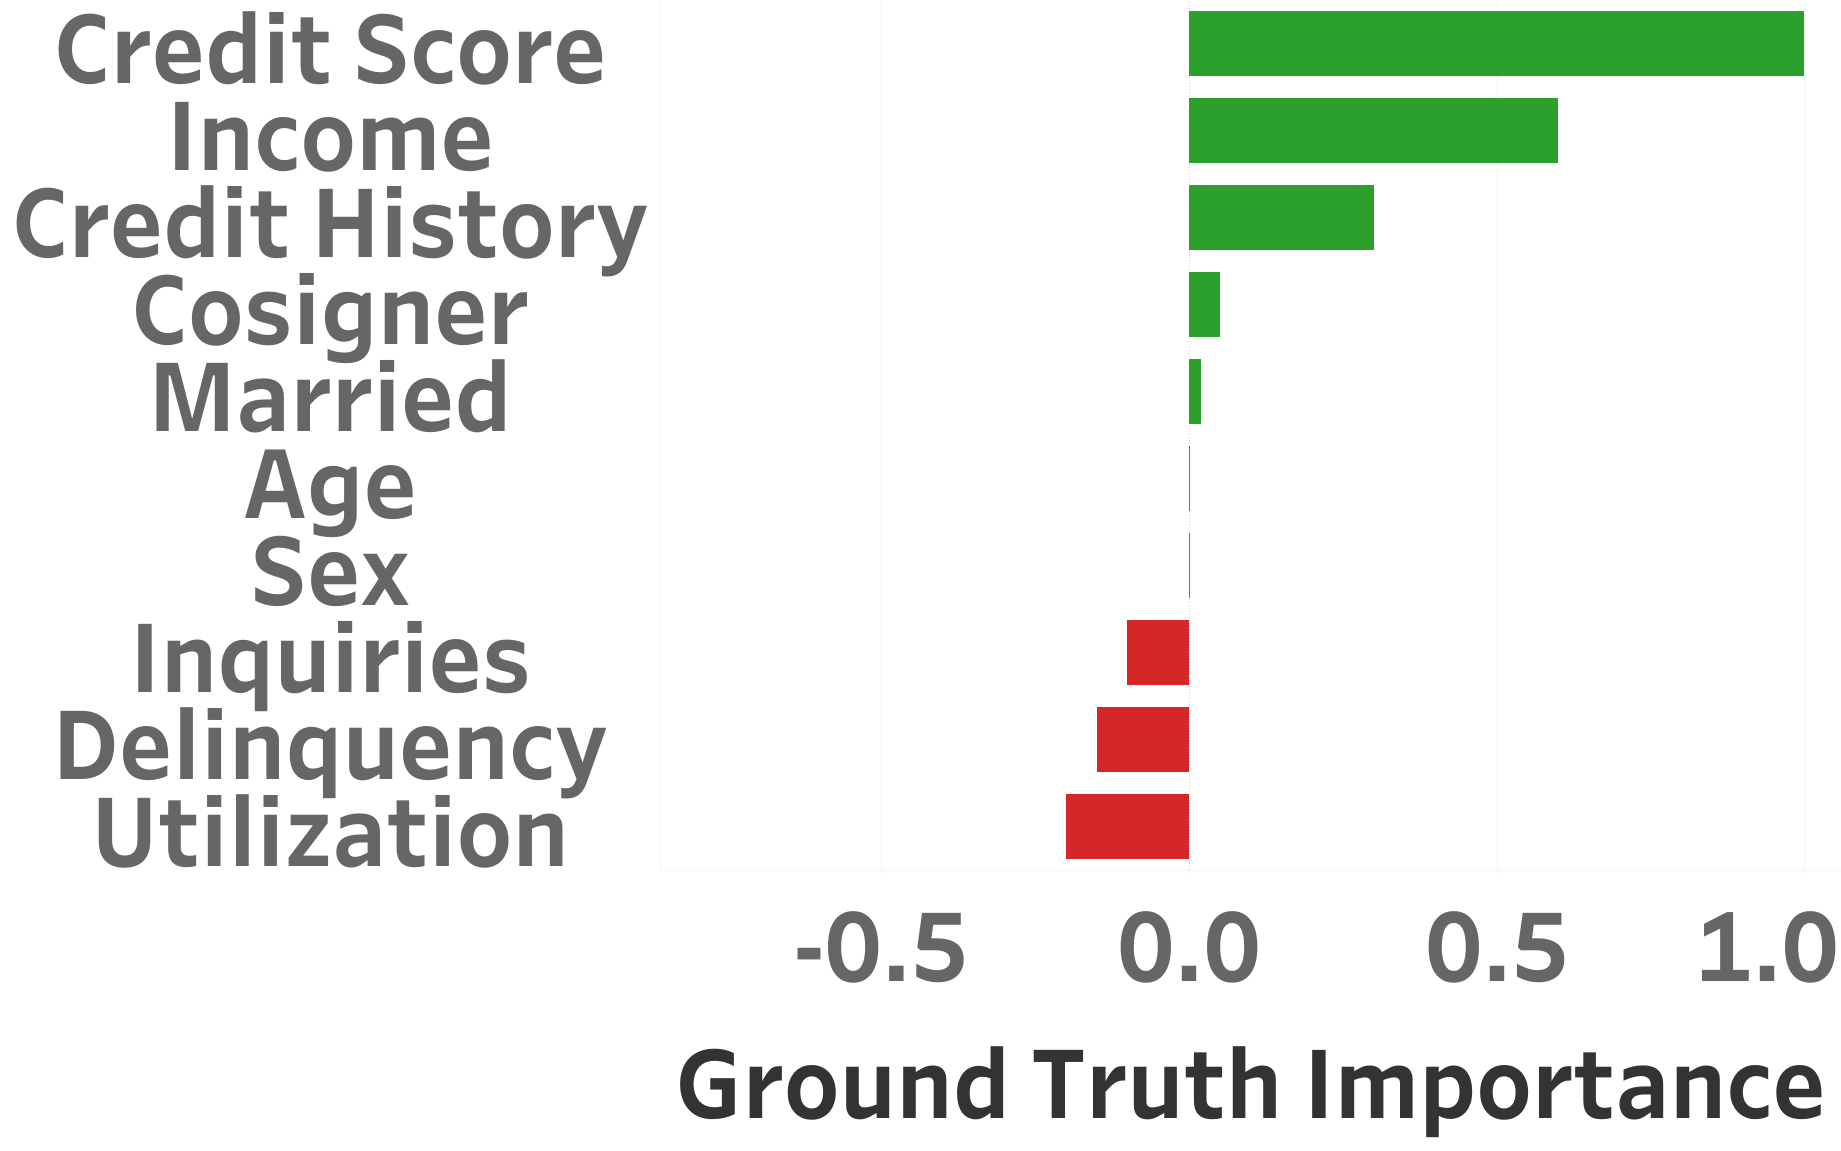
\includegraphics[width=\linewidth]{Figures/g_ex.png}
    \end{minipage}} & \multicolumn{3}{c}{\begin{minipage}{.3\textwidth}
      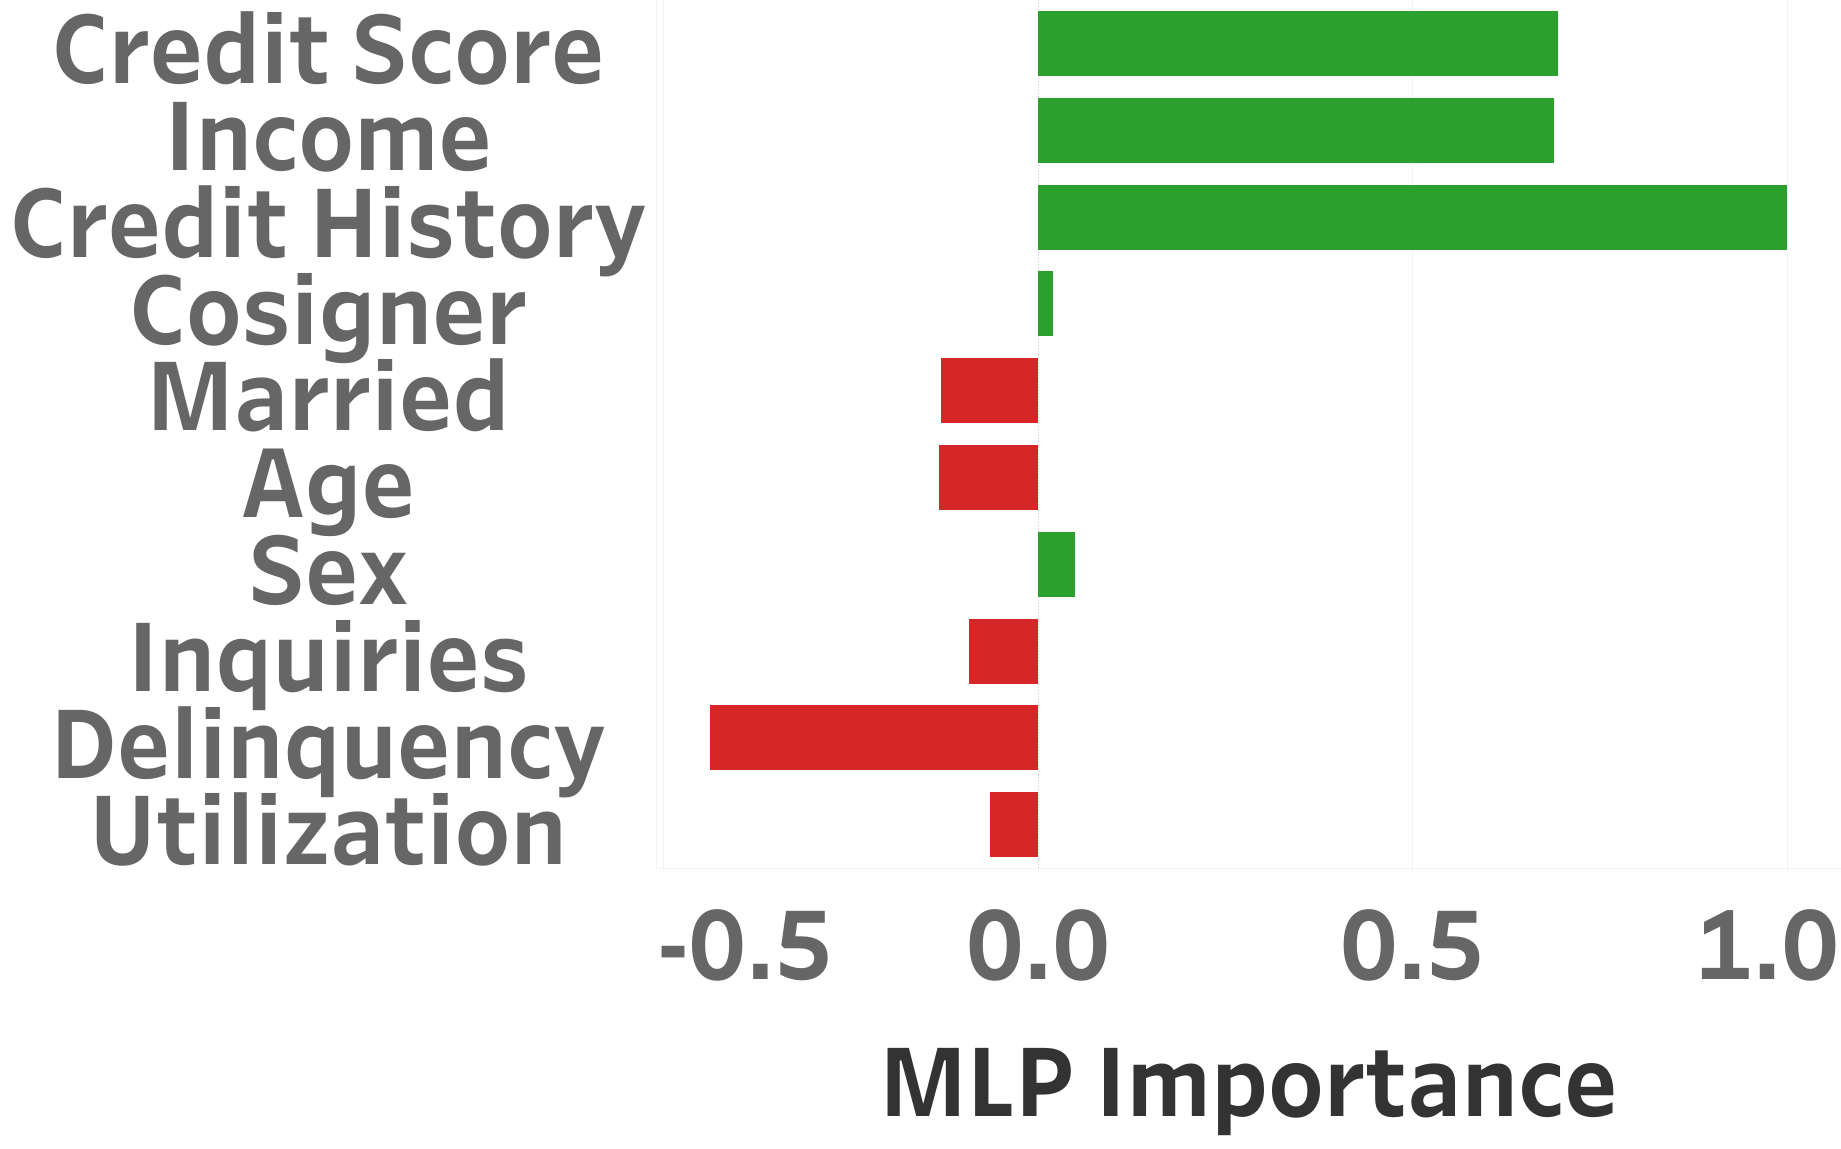
\includegraphics[width=\linewidth]{Figures/mlp_ex.png}
    \end{minipage}}  & \multicolumn{3}{c}{\begin{minipage}{.3\textwidth}
      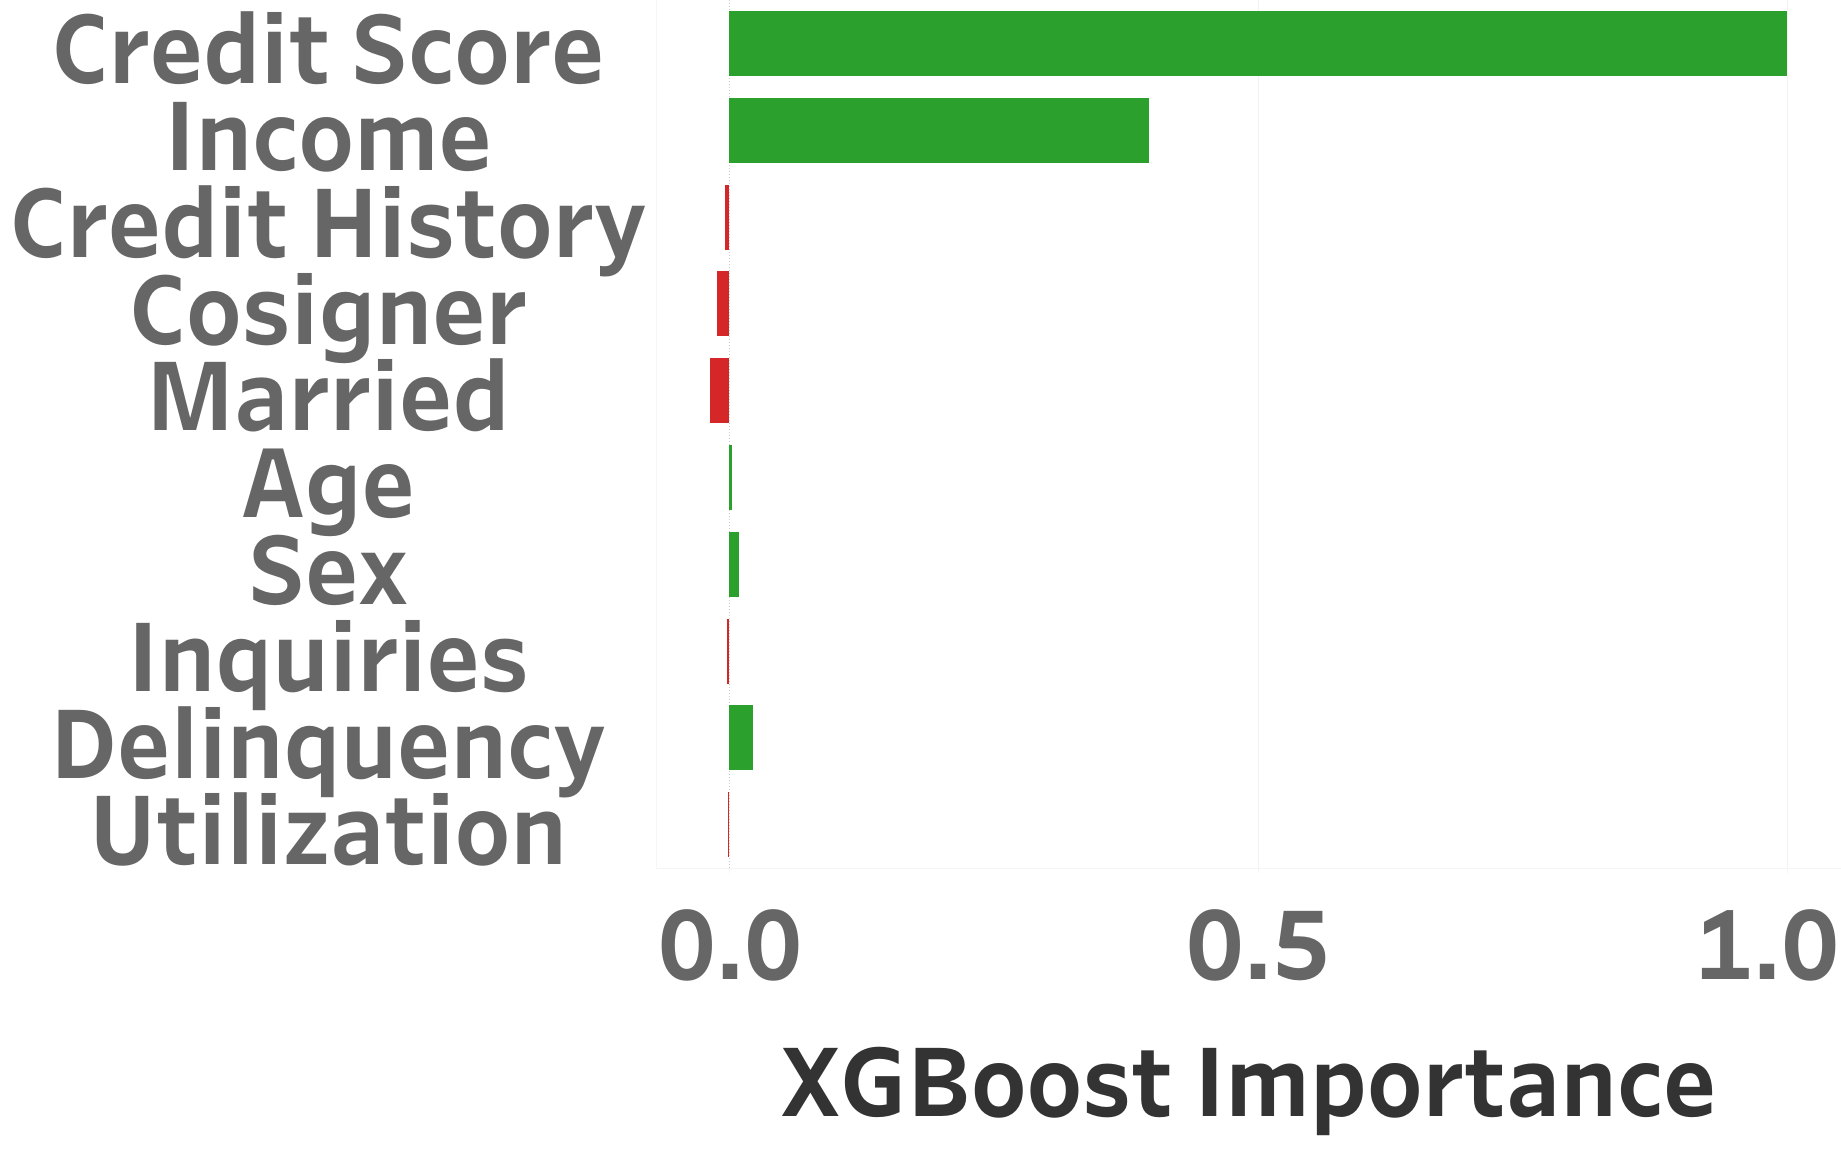
\includegraphics[width=\linewidth]{Figures/xgboost_ex.png}
    \end{minipage}} \tabularnewline %\midrule
\end{tcolorbox}
\noindent\begin{minipage}{\textwidth}
\captionof{figure}{Ground truth feature importance along with qualitatively different explanations for John obtained when using two instances of the pipeline. In the first pipeline, LIME is used to an MLP whereas in the second pipeline LIME is used to explain an XGBoost model. Feature importances are illustrated using diverging bar charts. }\label{box}
\end{minipage}

\item The concrete demonstration of the unfaithfulness and inconsistency of post hoc explainers in Figure \ref{box} motivates the main thrust of this paper. 
\end{itemize}

\section{Evaluation Metrics for LIME and SHAP}
    \label{sec:evaluation_metrics}
    \begin{itemize}
    \item Because feature importance values from LIME and SHAP indicate which features are important to $\mathcal{M}$ but not necessarily which features are important to $\mathcal{G}$, we need metrics that capture this difference.
    
    \item Before designing metrics, it is necessary to articulate what the ground truth actually is. 
            
    \item Instead of using direct comparisons like $\norm{\beta^{\text{LIME}} - \beta}_2$ or $\norm{\beta^{\text{SHAP}} \xi - \beta \xi}_2$, we will evaluate $\beta^{\text{LIME}}$ and $\beta^{\text{SHAP}}$ based on how they are used in practice. 
    
    \item To capture how well LIME and SHAP can do these things, we use three metrics. 
    \end{itemize}

\section{Unfaithfulness of Post Hoc Explanations}
    \label{sec:unfaithfulness}
    \begin{itemize}
    \item In this section, we investigate the causes of unfaithful explanations. Unfaithfulness can be measured in different ways. 
    
    \item First, we will evaluate the faithfulness of LIME and SHAP explanations of $\mathcal{M}$ with respect to $\mathcal{G}$ using the three metrics discussed in Section \ref{sec:evaluation_metrics}. 
    \end{itemize}

    \subsection{Evaluating Faithfulness}
        \label{sec:evaluating_faithfulness}
         Our goal is that evaluations using our three metrics will reveal ways that post hoc explanations could yield misleading insights.

        
                    
                    
        \paragraph{\textbf{Identifying Feature Importance Sign}}
            \label{sec:sign_acc}
            \begin{itemize}
            \item We first assess the faithfulness of LIME and SHAP by checking if the signs of the feature importance values obtained by inspecting the coefficients of their (underlying) models.
                        
                        
            \item Figure \ref{fig:lime_shap_sign_accs} shows a bar plot of the accuracies with which LIME and SHAP could identify the correct sign of each feature for 100 applicants in the test set.
            \end{itemize}
                    
        \paragraph{\textbf{Ranking Features Correctly}}
            \label{sec:feature_rankings}
            \begin{itemize}
            \item Using feature importance values from LIME and SHAP and the coefficient values from $\mathcal{G}$ in Equation \ref{eqn:gt}, we can produce pairs of rankings of the features from most harmful to loan approval to most beneficial to loan approval and then check how correlated are to tell how faithful the explainers' rankings were to $\mathcal{G}$.
            
            \item Figure \ref{fig:lime_shap_Spearman_signed} shows violin plots of the Spearman correlations for LIME and SHAP rankings of the 100 applicants.
            \end{itemize}
            
        \paragraph{\textbf{Recall of the Most Important Features}}
            \label{sec:recall}
            \begin{itemize}
            \item The previous experiments explored the ability of LIME and SHAP to recover correct importance information about all features used by $\mathcal{G}$, but in practice,  users may only care about, say, the top five most important features.
            
            \item The results are shown in Figure \ref{fig:avg_recall} using line plots.
            \end{itemize}

    


        \begin{figure}[ht!]
            \centering
            \begin{subfigure}[t]{.3\textwidth}
              \centering
              \captionsetup{justification=centering}
                  \raisebox{.2cm}{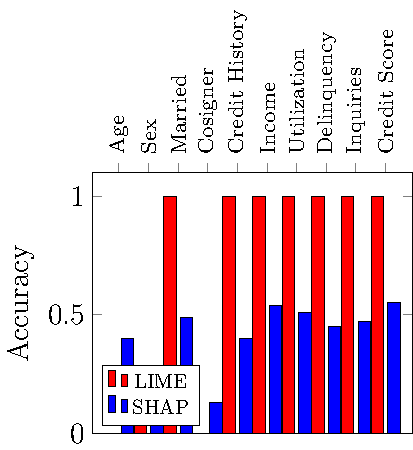
\includegraphics[width=\textwidth]{FinalFigures/sec4_1_sign_accs_final.pdf}}%{Figures/lime_shap_Spearman_magnitude.png}

              \caption{Sign Prediction Accuracy}%Spearman rank correlations of feature importance magnitudes from LIME and SHAP against the true ranking from $\mathcal{G}$. }
               \label{fig:lime_shap_sign_accs}
            \end{subfigure}%
            \hfill
            \begin{subfigure}[t]{.3\textwidth}
              \centering
               \captionsetup{justification=centering}
              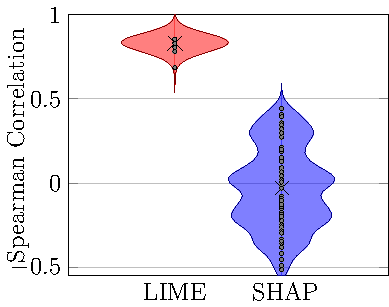
\includegraphics[width=\textwidth]{FinalFigures/sec4_1_spearmans_final.pdf}%{Figures/lime_shap_Spearman_signed.png}
              \caption{Importance rankings}%Spearman rank correlations of signed feature importance from LIME and SHAP against the true ranking from $\mathcal{G}$.}
               \label{fig:lime_shap_Spearman_signed}
            \end{subfigure}
            \hfill
            \begin{subfigure}[t]{.3\textwidth}
              \centering
               \captionsetup{justification=centering}
            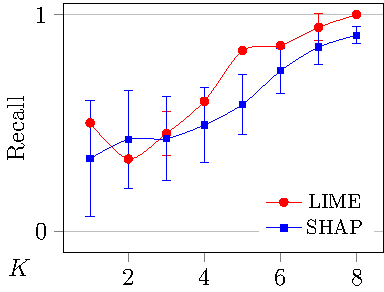
\includegraphics[width=\textwidth]{FinalFigures/sec4_1_recalls_final.pdf}%
            \caption{Recall}%The average and standard error of recall of LIME and SHAP when attempting to capture the top K most important features to $\mathcal{G}$ when explaining $\mathcal{M}$, for varied $K=1,2,3,...$ number of features.}
            \label{fig:avg_recall}
            \end{subfigure}
            \caption{Violin plots of Spearman correlations between LIME and SHAP feature importance rankings, both signed and unsigned, against the true rankings (left and middle), along with the average and standard error of $recall_K$ when attempting to capture the top $K$ most important features to $\mathcal{G}$ by explaining $\mathcal{M}$ with LIME and SHAP.}
           \label{fig:lime_shap_Spearman_signed_mag_recall}
        \end{figure} 
        
            Our experiments showed that LIME and SHAP explanations of an accurate MLP always had some errors. 

    % REWORK THE FLOW OF THIS PART
    \subsection{Causes of Unfaithful Explanations}
        \begin{itemize}
        \item Since researchers usually do not have access to their data's ground truth $\mathcal{G}$, any efforts toward producing explanations of a black box that reflect $\mathcal{G}$ faithfully must be supported by additional assumptions on the data and $\mathcal{M}$.

        T\item he necessity of causal inference conditions is especially important for business research because faithful and interesting business insights are preferably causal relations.

        
        \item To demonstrate the effect of correlation and confounding on explanations, we will compare the explanation quality of models trained in three scenarios. 
        
        \item Unlike the dataset used in Section \ref{sec:unfaithfulness} which was based off of a ground truth designed to model loan approval realistically, the control dataset is generated by a simple ground truth model that determines loan approval from five independent features.
        
        \item Our experiments show that even when explaining a model $\mathcal{M}$ trained with independent features
        %after eliminating causal inference condition violations, 
        LIME and SHAP's of $\mathcal{M}$ are sometimes not completely faithful to $\mathcal{G}$. 
        \end{itemize}
    %use fbox to tailor crop
    \begin{figure}[ht!]
    \centering
        \begin{subfigure}{.3\textwidth}
        \centering
        \raisebox{.2cm}{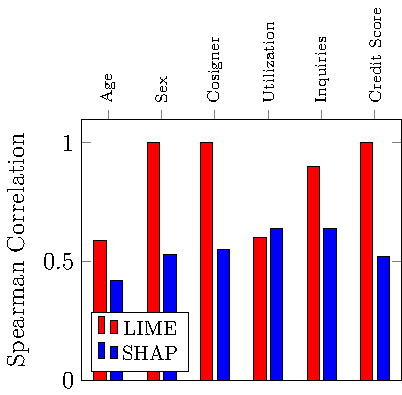
\includegraphics[width=\textwidth]{FinalFigures/sec4_3_perfect_data_sign_accs_final.pdf}}
        \caption{Importance Sign Accuracy}
        \label{fig:perfect_dataset_sign_accs}
        \end{subfigure}%
        \hfill
        \begin{subfigure}{.3\textwidth}
        \centering
        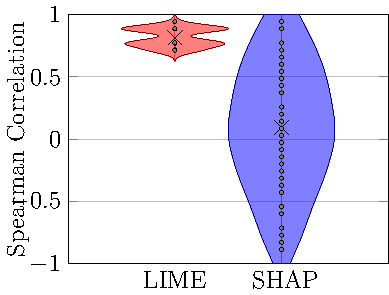
\includegraphics[width=\textwidth]{FinalFigures/sec4_3_perfect_data_spearmans_final.pdf}
        \caption{Importance Ranking}
        \label{fig:perfect_dataset_spearmans}
        \end{subfigure}
        \hfill
        \begin{subfigure}{.3\textwidth}
        \centering
        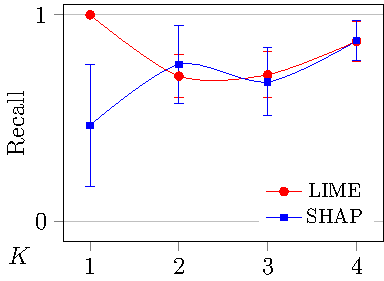
\includegraphics[width=\textwidth]{FinalFigures/sec4_3_perfect_data_recalls_final.pdf}
        \caption{Recall}
        \label{fig:perfect_dataset_recalls}
        \end{subfigure}
    \caption{LIME and SHAP performance when explaining an MLP with accuracy $\sim .85$ and AUC $\sim .95$ trained on a dataset with independent, unconfounded features, and no unobserved features}
               \label{fig:perfect_dataset}
    \end{figure}

    \paragraph{\textbf{Correlated Features}}
        To show how it can be difficult to distinguish the importance of correlated features, we utilize a modification of the control dataset where the credit score feature becomes a function of age. 
            %We construct $\mathcal{G}_{colinear}$ by altering $\mathcal{G}^*$ such that credit score becomes a function of age:
        %http://www.themoneyalert.com/credit-score-rating-scale-range/
            % np.random.normal(550,20) + 1.9 * X['Age'] +  np.sin(X['Age'])
            \begin{equation*}
                \text{credit score} = 1.9 \cdot \text{Age} + sin(\text{Age}) + \epsilon,
            \end{equation*}
        \noindent where $\epsilon \sim \mathcal{N}(550, 20)$. This model reflects that, on average, credit scores increase with age.
        
        Figure \ref{fig:lime_shap_colinear} shows pairs of violin plots illustrating how feature rankings from both LIME and SHAP are generally more faithful when they get to explain models trained on data with independent features.
        
    %\tw{I would also investigate the importance of credit score and age, since these two features are correlated. I would show whether the ranking of the two features increased or decreased because of the collinearity} \textcolor{blue}{done: see figures 9a-d}
            \begin{figure}[ht!]
                \centering
                \begin{subfigure}{.3\textwidth}
                  \centering
                  \captionsetup{justification=centering}
                  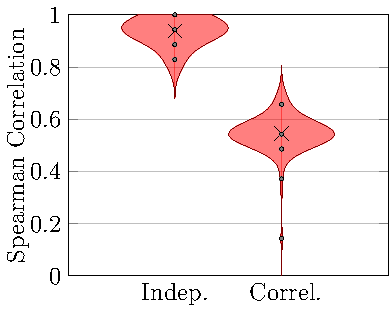
\includegraphics[width=\textwidth]{FinalFigures/sec4_3_corr_lime_spearmans_final.pdf}%{Figures/lime_spearman_colinear.png}
                                %\includegraphics[width=.9\linewidth]{Figures/lime_shap_Spearman_magnitude.png}
    
                  \caption{LIME}%Spearman rank correlations of ranked feature importance magnitudes from LIME against the true ranked magnitudes from $\mathcal{G}$.}
                   \label{fig:lime_colinear}
                \end{subfigure}%
                \hspace{3cm}
                \begin{subfigure}{.3\textwidth}
                  \centering
                     \captionsetup{justification=centering}
                  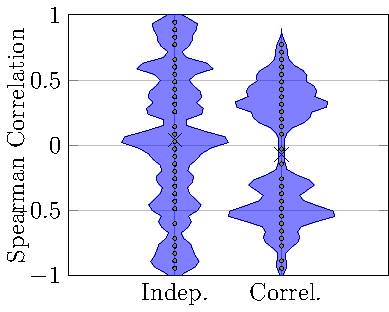
\includegraphics[width=\textwidth]{FinalFigures/sec4_3_corr_shap_spearmans_final.pdf}%{Figures/shap_spearman_colinear.png}
    
                  %\includegraphics[width=.9\linewidth]{Final_Figures/fig9b.png}%{Figures/shap_spearman_colinear.png}
                  \caption{SHAP}%Spearman rank correlations of signed feature importance magnitudes from LIME and SHAP against the true ranking from $\mathcal{G}$.}
                   \label{fig:shap_colinear}
                \end{subfigure}
                
                \caption{Violin plots of 100 Spearman rank correlations of feature importance rankings when explaining models $\mathcal{M}$ trained on $\mathcal{G}^*$ and $\mathcal{G}_{\text{colinear}}$, respectively}
                \label{fig:lime_shap_colinear}
            \end{figure}
    

            
    
    \paragraph{\textbf{Confounded Features}}
        \begin{itemize}
        \item Confounding is a more difficult phenomenon to deal with in the pipeline than correlation because while it is simple to check if two features are correlated, it is impossible to test if a feature is confounded. 
        % should I combine the analysis?
        
        \item We begin with the case of unobserved confounding. 

        \item Figure \ref{fig:lime_shap_obs_conf} illustrates the harmful effect of observed confounding by contrasting the faithfulness of the LIME and SHAP explanations of a model trained on a dataset with an observed confounded with those of a model trained on the control dataset.
            
            
        \item Without knowing the causal relations underlying the dataset, observed confounding cannot be distinguished from correlation. 

            \begin{figure}[ht!]
                \centering
                \begin{subfigure}{.3\textwidth}
                  \centering
                  \captionsetup{justification=centering}
                  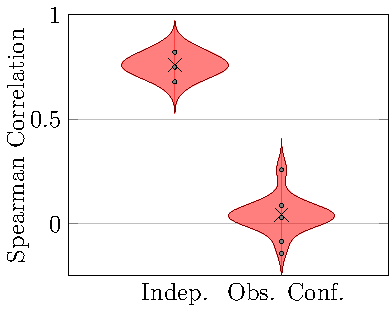
\includegraphics[width=\textwidth]{FinalFigures/sec4_3_lime_obsconf_spearmans_final.pdf}
                  \caption{LIME}
                   \label{fig:lime_obs_conf}
                \end{subfigure}%
                \hspace{3cm}
                \begin{subfigure}{.3\textwidth}
                  \centering
                     \captionsetup{justification=centering}
                  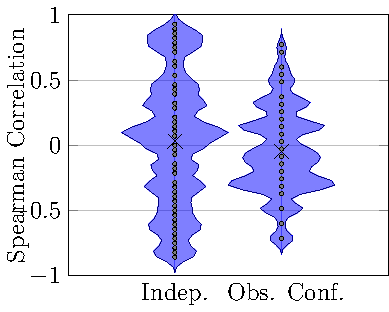
\includegraphics[width=\textwidth]{FinalFigures/sec4_3_shap_obsconf_spearmans_final.pdf}
                  \caption{SHAP}
                   \label{fig:shap_obs_conf}
                \end{subfigure}
                
                \caption{Violin plots of 100 Spearman rank correlations of feature importance rankings when explaining models $\mathcal{M}$ trained on $\mathcal{G}^*$ and $\mathcal{G}_{\text{observed confounding}}$, respectively}
                \label{fig:lime_shap_obs_conf}
            \end{figure}
            
           \item  A dataset has an unobserved confounding problem when an unobserved feature is a causal driver of the target variable and some observed feature. 


            \begin{figure}[ht!]
                \centering
                \begin{subfigure}{.3\textwidth}
                  \centering
                  \captionsetup{justification=centering}
                  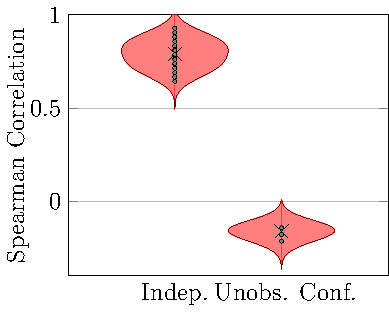
\includegraphics[width=\textwidth]{FinalFigures/sec4_3_lime_unobsconf_spearmans_final.pdf}
                  \caption{LIME}
                   \label{fig:lime_unobs_conf}
                \end{subfigure}%
                \hspace{3cm}
                \begin{subfigure}{.3\textwidth}
                  \centering
                     \captionsetup{justification=centering}
                  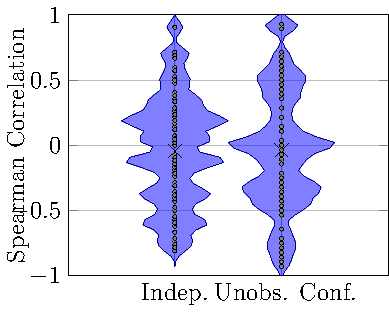
\includegraphics[width=\textwidth]{FinalFigures/sec4_3_shap_unobsconf_spearmans_final.pdf}
                  \caption{SHAP}
                   \label{fig:shap_unobs_conf}
                \end{subfigure}
                
                \caption{Violin plots of 100 Spearman rank correlations of feature importance rankings when explaining models $\mathcal{M}$ trained on $\mathcal{G}^*$ and $\mathcal{G}_{\text{unobserved confounding}}$, respectively}
                \label{fig:lime_shap_unobs_conf}
            \end{figure}
        \end{itemize}


\section{Inconsistency of Post Hoc Explanations}
    \label{sec:inconsistency}
        \begin{itemize}
         \item Inconsistency of post hoc explainers refers to situations in which one or more post hoc explainers provide a set of explanations that contains some internal disagreement. 

        % should i mention that the dataset matters?
        \item Explanation inconsistency has to do with the \textit{model being explained} (i.e., $\mathcal{M}$) and the \textit{explainers} (that is, $\mathcal{E})$. 
         
         \item We showcase in the following subsections different causes of inconsistency in each stage of the pipeline. 

         \end{itemize}

    
    \subsection{Stage 1 Issues: Diversity of Decision Boundaries for $\mathcal{M}$}
        \label{sec:rashomon_overfitting}
        
        Explanations of a model are governed by that model's decision boundary. 

        % put this first per dr. wang's request
        % talk about model performance and rashomon mayble?
         \paragraph{\textbf{Inconsistency from Explaining Different Models}}
         \begin{itemize}
        \item Despite being trained on the same data and attaining approximately the same predictive performance, explanations of two distinct models with different decision boundaries will necessarily be different. 

        % DOUBLE CHECK THE SHAP RESULT
        \item We show this in further generality by checking how correlated the feature rankings of 100 applicants are for LIME and SHAP explanations of two pairs of models, all with AUC$\simeq .85$.


        \begin{figure*}[ht!]
        \centering
            \begin{subfigure}[t]{0.45\textwidth}
            \centering
            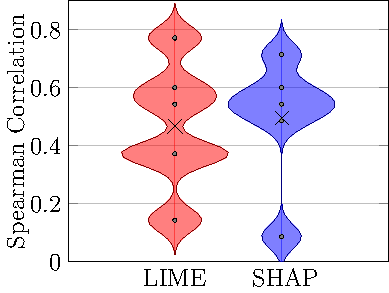
\includegraphics[width=.73\textwidth]{FinalFigures/sec5_2_incon_mlp_xgb_final.pdf}
            \caption{Correlation between LIME and SHAP explanations of pairs of explanations from an MLP and XGBoost model, respectively} \label{fig:mlp_xgb_corr}
        \end{subfigure}
        \hspace{1cm}
        \begin{subfigure}[t]{0.45\textwidth}
            \centering
            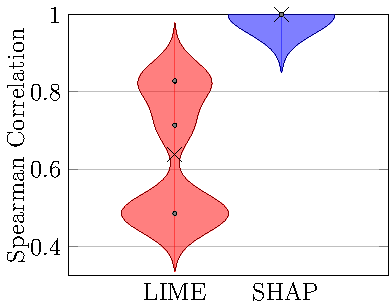
\includegraphics[width=.73\textwidth]{FinalFigures/sec5_2_incon_xgb_xgb_final.pdf}
            \caption{Correlation between LIME and SHAP explanations of pairs of explanations from two distinct XGBoost models} \label{fig:xgb_xgb_corr}
        \end{subfigure}
        \caption{Violin plots of Spearman correlations between pairs of explanations of different combinations of black box models}
        \label{fig:model_corrs}
        \end{figure*}
        \end{itemize}

          \paragraph{\textbf{Instability Due to Decision Boundary Volatility}}          
          \begin{itemize}
         \item Intuitively, explanations for the outcomes occuring in similar scenarios should be similar as well. 
          
         \item To demonstrate instability, we construct another loan approval model based only on income and credit utilization and check the instability of LIME's coefficients when overfitting is and is not present.

         \item Figure \ref{fig:dbd_dists} shows that explainers for $\mathcal{M}_{\text{overfit}}$ are more unstable than those for $\mathcal{M}$.
         \end{itemize}

            \begin{figure}[ht!]
                \centering
                \begin{subfigure}[t]{.3\textwidth}
                  \centering
                  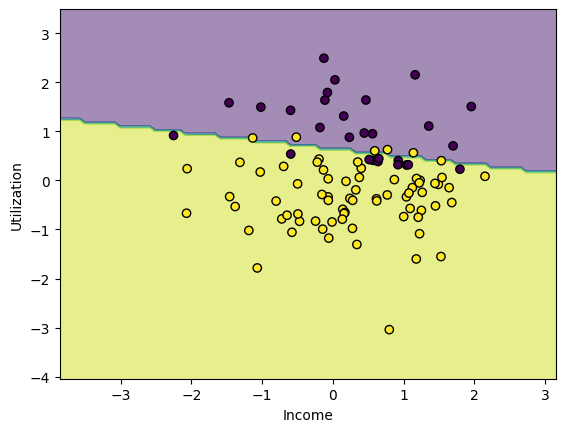
\includegraphics[width=\textwidth]{Figures/dbd_M.png}
                  \caption{Decision boundary of $\mathcal{M}$}
                  \label{fig:M_dbd}
                \end{subfigure}%
                \hfill
                \begin{subfigure}[t]{.3\textwidth}
                  \centering
                  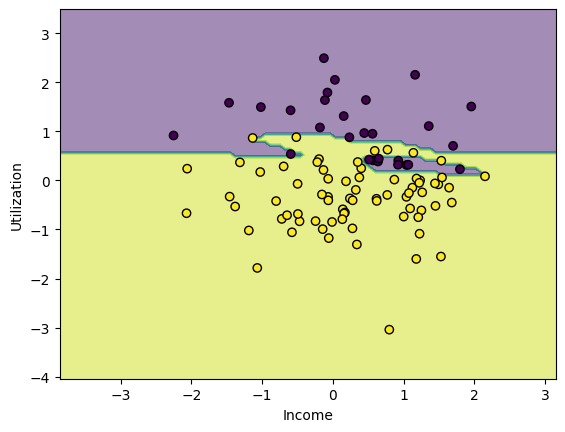
\includegraphics[width=\textwidth]{Figures/dbd_Mp.png}
                  \caption{Decision Boundary of $\mathcal{M}_{\text{overfit}}$}
                  \label{fig:Mp_dbd}
                \end{subfigure}
                \hfill
               \begin{subfigure}[t]{.3\textwidth}
                \centering
                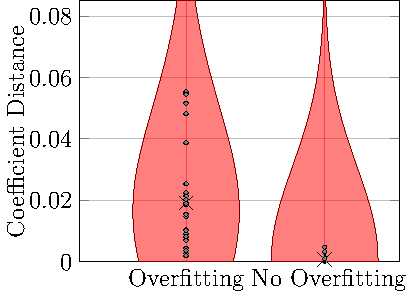
\includegraphics[width=\textwidth]{Figures/sec5_1_overfitting_spearmans.pdf}%{Figures/dbd_dists.png}
                \caption{Effect of overfitting on stability}%Violin plots representing the stability of explainers of $\mathcal{M}$ and $\mathcal{M}_{\text{overfit}}$}
                \label{fig:dbd_dists}
                \end{subfigure}
                \caption{Visualizations of decision boundaries for MLPs that do and do not overfit ($\mathcal{M}$ and $\mathcal{M}_{\text{overfit}}$) on a simple two variable loan approval dataset along with violin plots representing the stability of explainers of $\mathcal{M}$ and $\mathcal{M}_{\text{overfit}}$. Yellow points are accepted applicants and purple points are denied applicants.}
                \label{fig:dbds}
            \end{figure}
            
    \subsection{Stage 2 Issues: Inconsistency Between and Within Explainers}
        \label{sec:conflict_between_within}
            Trusting and justifying post hoc explanations can be difficult because different explanations can be obtained for the same input to the same black box model.
            
            \paragraph{\textbf{Inconsistency Between Explainers}}
                We suppose that business researchers using tabular data would be likely to try both LIME and SHAP due to their popularity, and so we test how often and to what extent their explanations of an XGBoost model agree. 
    
    \paragraph{\textbf{Inconsistency From The Same Explainer}}
           In addition to different explainers disagreeing with each other, it is unfortunately also the case that individual explainers can produce a set of explanations for the same input that has some internal disagreement. 

  
\begin{figure*}[ht!]
\centering
    \begin{subfigure}[t]{0.45\textwidth}
    \centering
    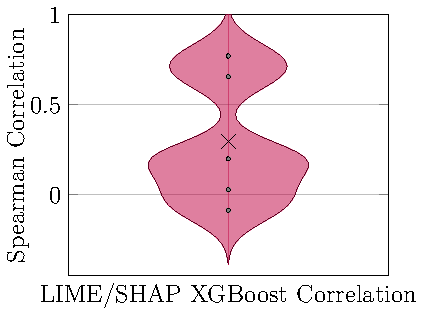
\includegraphics[width=.73\textwidth]{FinalFigures/sec5_2_incon_lime_shap_xgb_final.pdf}
    \caption{Correlation between LIME and SHAP explanations of pairs of explanations the same XGBoost model} \label{fig:lime_shap_xgb_corr}
\end{subfigure}
\hspace{1cm}
\begin{subfigure}[t]{0.45\textwidth}
    \centering
    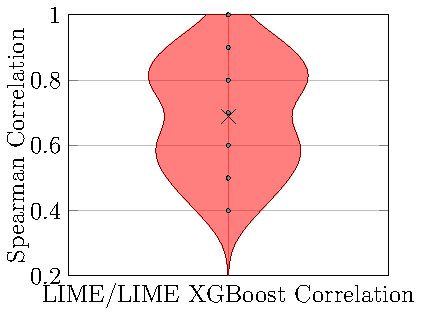
\includegraphics[width=.73\textwidth]{FinalFigures/sec5_2_incon_lime_lime_xgb_final.pdf}
    \caption{Correlation explanations of pairs of explanations of the same XGBoost model from two distinct LIME explainers} \label{fig:lime_lime_xgb_corr}
\end{subfigure}
\caption{Violin plots of Spearman correlations between pairs of explanations of one black box model from different combinations of explainers}
\label{fig:explainer_corrs}
\end{figure*}

\section{Theoretical Considerations For Mitigations}
    \label{sec:theoretical_considerations}
    We will present several theoretical results which serve a dual purpose of motivating mitigation strategies that aid recovery of $\beta$ and representing how faithful LIME and SHAP explanations can be in simple conditions. 
    
        \subsection{$\beta^\text{LIME}$ when Explaining a Linear Model}
            \label{sec:lime_linear_case}
            \begin{itemize}
             \item The behavior of LIME variants depends on 1) whether feature discretization is used, 2) how data are sampled, 3) the sample weighting function $\pi$, and 4) whether sparsity regularization is used. 
            
             \item Theorem 1, which is proven in the Appendix, proves that under our assumptions $\beta^{\text{LIME}}$ converges to $\beta$ in the large $N$ limit when explaining a linear model $\beta x$.
             
            \item Feature importance measures that directly estimate $\beta$, like standard regression and LIME's in this case, are said to represent the theoretical importance of each feature \citep{AchenChristopherH1982Iaur}. 

            \end{itemize}
            
         \subsection{$\beta^\text{SHAP}$ when Explaining a Linear Model}
            \begin{itemize}
              \item SHAP does \emph{not} recover $\beta$ and should not be relied upon for this purpose. The importance of the $i^{th}$ feature of the $n^{th}$ data sample $x^{(n)}_i$ in a SHAP explanation is the data sample's Shapley value, which reduces to the following when SHAP is used to explain a linear model. 
             \begin{equation}
                \label{eqn:shap_gt}
                \beta_i^\text{SHAP} = \beta_i (x^{(n)}_i - \bar{x}_i)
             \end{equation}
             according to ~\citep{lundberg17shap}.
             
             \item  Unlike LIME, SHAP estimates the situational importance~\citep{StrumbeljErik2014Epma} for a feature. 
             \end{itemize}

            \begin{theorem}
                \label{thm:lime_thm}
                Suppose $f:\mathbb{R}^D\rightarrow \mathbb{R}$ that maps $\mathbf{x} \mapsto \beta^T \mathbf{x}$ is explained at a sample $\xi$ drawn from $\mathcal{N}(\mathbf{0}, \mathds{1}_D)$ with LIME. Let LIME use a generalized ridge regressor as a surrogate model with sparsity penalty parameter $\lambda=1$ and shrinkage target equal to $\mathbf{0}_D$. Suppose further that LIME uses all features in the explanation, does not discretize them, samples $N$ i.i.d. data points $\mathbf{x} \sim \mathcal{N}(\xi, \mathds{1}_D)$, and weights those samples with the exponential kernel $\pi(\mathbf{\xi},\mathbf{x}) = exp(-\norm{\mathbf{\xi}-\mathbf{x}}_2^2/2\nu^2)$ using bandwidth $\nu>0$. Then, in the large $N$ limit, the coefficients of LIME converge to $\beta$. That is,
                \begin{equation*}
                    \beta^{\text{LIME}} \rightarrow \beta
                \end{equation*}
                as $N \rightarrow \infty$.
            \end{theorem}

            \begin{proposition}
                Under the assumptions of Theorem 1, solutions to LIME's ridge regression problems satisfy the following bound. Let the $N$ samples generated by LIME be collected into a data matrix $\mathbf{X}\in\mathbb{R}^{N\times D}$ and $\mathbf{W}\in\mathbb{R}^{N\times N}$ be the ridge regression weight matrix with $w_{nn} = \pi(\mathbf{\xi},\mathbf{x}^{(n)})$ for $n=1,\ldots,N$ and 0 elsewhere. Define the shorthand notation $\mathbf{A}:= \mathbf{X}^T \mathbf{W}\mathbf{X}$ so that the ridge regression solution is
                \begin{equation*}
                    \beta^{\text{LIME}} = (\mathbf{A} + \mathbf{I})^{-1}\mathbf{A} \beta
                \end{equation*}
                Then
                \begin{equation*}
                    \frac{\sigma_{\max}(\mathbf{A})}{\sigma_{\max}(\mathbf{A}) + 1} \leq \norm{(\mathbf{A} + \mathbf{I})^{-1}\mathbf{A}} \leq \frac{\sigma_{\max}(\mathbf{A})}{\sigma_{\min}(\mathbf{A}) + 1}
                \end{equation*}
                where $\sigma_{\min}(\mathbf{A})$ and $\sigma_{\max}(\mathbf{A})$ are the smallest and largest singular values of $\mathbf{A}$, respectively. 
            \end{proposition}
        
            \begin{corollary}
                Under the assumptions of Theorem 1, with fixed finite $N$, taking $\nu \rightarrow 0$ causes $\beta^{\text{LIME}} \rightarrow \mathbf{0}$. 
            \end{corollary}
            
            \begin{corollary}
                Under the assumptions of Theorem 1, with fixed finite $N \gg 1$ and $\nu\rightarrow \infty$, taking $\nu \rightarrow 0$ causes $\beta^{\text{LIME}} \rightarrow \beta$. 
            \end{corollary}

                %It remains to demonstrate the existence of $L$ and derive its value.
            \begin{theorem}
                \label{thm:shap_thm}
                Suppose $f:\mathbb{R}^D\rightarrow \mathbb{R}$ that maps $\mathbf{x} \mapsto \beta^T \mathbf{x}$ is explained with SHAP and $\mathbf{x} \sim \mathcal{N}(0, \mathbf{1}_D)$. Then there exists $C\in \mathbb{R}$ such that $\beta^{\text{SHAP}} = C \beta \xi$ for all $\xi \sim \mathcal{N}(0, \mathbf{1}_D)$. 
            \end{theorem}


\section{Mitigation Strategies}
    In this section, we use the results of our experiments and the implications of the theoretical results from Section \ref{sec:theoretical_considerations} to propose and test some mitigation strategies for unfaithfunless and inconsistency.

    \subsection{Attempted ``Mitigation'' Strategies for Unfaithfulness}
    \label{sec:incorrectness_mitigation} %\textcolor{red}{move this to the end of section 4. this is the mitigation strategy for incorrectness}
        We propose a few intuitive mitigation strategies for explanation faithfulness based on data preprocessing and, model training, and explainer hyperparameters. We first demonstrate the truth of Corrolaries 1 and 2 from Section \ref{sec:theoretical_considerations}.

        \subsubsection{Increasing $\nu$ and $N$ for LIME } 
    \label{sec:lime_params}
    Corollaries 1 and 2 from Section \ref{sec:theoretical_considerations} imply that LIME's kernel bandwidth $\nu$ and number of perturbed samples $N$ need to be large in order for $\beta^{\text{LIME}}$ to be close to $\beta$, so this Section will experiment with how their respective sizes affect explanation quality. 
            \begin{figure}[ht!]
                \centering
                \begin{subfigure}[t]{.3\textwidth}
                  \centering
                  \captionsetup{justification=centering}
                      \raisebox{.2cm}{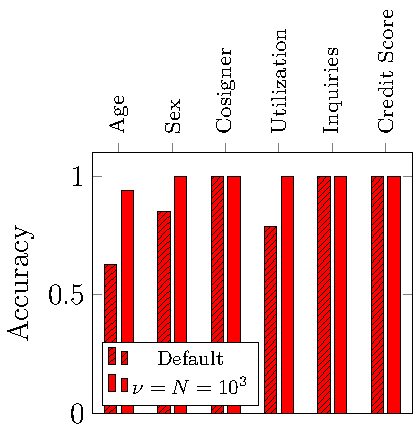
\includegraphics[width=\textwidth]{Figures/sec4_4_lime_sign_accs.pdf}}%{Figures/lime_shap_Spearman_magnitude.png}
    
                  \caption{Sign Prediction Accuracy}%Spearman rank correlations of feature importance magnitudes from LIME and SHAP against the true ranking from $\mathcal{G}$. }
                   \label{fig:lime_tuning_sign_accs}
                \end{subfigure}%
                \hfill
                \begin{subfigure}[t]{.3\textwidth}
                  \centering
                   \captionsetup{justification=centering}
                  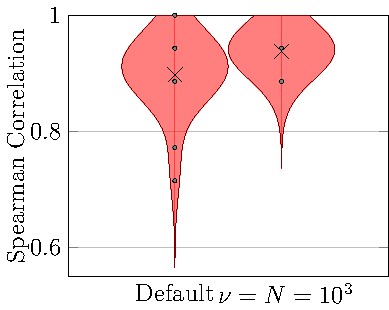
\includegraphics[width=\textwidth]{Figures/sec4_4_lime_spearmans.pdf}%{Figures/lime_shap_Spearman_signed.png}
                  \caption{Importance rankings}%Spearman rank correlations of signed feature importance from LIME and SHAP against the true ranking from $\mathcal{G}$.}
                   \label{fig:lime_tuning_spearmans}
                \end{subfigure}
                \hfill
                \begin{subfigure}[t]{.3\textwidth}
                  \centering
                   \captionsetup{justification=centering}
                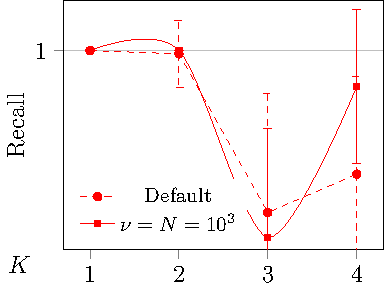
\includegraphics[width=\textwidth]{Figures/sec4_4_lime_recalls.pdf}%
                \caption{Recall}%The average and standard error of recall of LIME and SHAP when attempting to capture the top K most important features to $\mathcal{G}$ when explaining $\mathcal{M}$, for varied $K=1,2,3,...$ number of features.}
                \label{fig:lime_tuning_recalls}
                \end{subfigure}
                \caption{Violin plots of Spearman correlations between LIME and SHAP feature importance rankings, both signed and unsigned, against the true rankings (left and middle), along with the average and standard error of $recall_K$ when attempting to capture the top $K$ most important features to $\mathcal{G}$ by explaining $\mathcal{M}$ with LIME and SHAP.}
               \label{fig:lime_tuning}
            \end{figure} 
    
        
    
        \subsubsection{Increasing AUC of $\mathcal{M}$}
        \label{sec:m_fidelity}
        \begin{itemize}
        \item Intuitively, holding the ability of a post hoc explainer to accurately explain models $\mathcal{M}$ constant, explanations of increasingly accurate models should be increasingly faithful to the ground truth. 
        
       \item Following intuition, both Figures \ref{fig:main_lime_M_auc_inc} and \ref{fig:main_shap_M_auc_inc} show a general positive trend between the AUC of $\mathcal{M}$ and the faithfulness and consistency of feature rankings. 
        \end{itemize}
    \begin{figure*}[!h]
    \centering
        \begin{subfigure}[t]{0.3\textwidth}
        \centering
        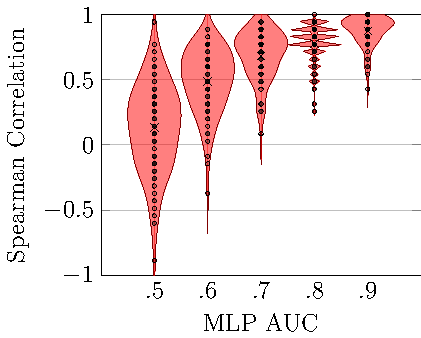
\includegraphics[width=\textwidth]{Figures/sec4_4_mlp_auc_lime.pdf}%{Figures/mag_vs_acc.pdf}
        \caption{LIME} \label{fig:main_lime_M_auc_inc}
    \end{subfigure}\hspace{3cm}
    \begin{subfigure}[t]{0.3\textwidth}
        \centering
        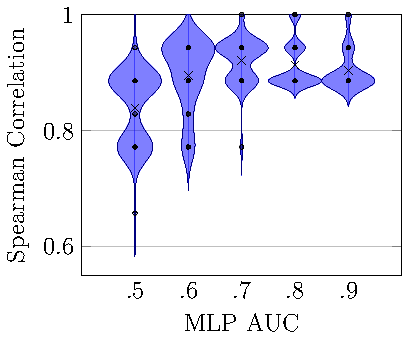
\includegraphics[width=\textwidth]{Figures/sec4_4_mlp_auc_avg_shap.pdf}%{Figures/signed_vs_acc.pdf}
        \caption{SHAP} \label{fig:main_shap_M_auc_inc}
    \end{subfigure}
    \caption{Spearman rank correlations of feature importance rankings for MLPs with varied AUC}
    \label{fig:acc_increase}
    \end{figure*}


        \subsubsection{Near Perfect Test Set Accuracy of Model Trained on Ideal Dataset}
        \label{sec:optimal_conditions}
        \begin{itemize}
        \item This section asks whether explanations from LIME and SHAP are perfect when the conditions for their use are practically ideal in the sense that 1) $\mathcal{M}$ has very high test set AUC and 2) the data set satisfies the causal inference conditions. 
    
        \item We repeat the experiments of Section \ref{sec:evaluating_faithfulness} once more, but this time explain the aforementioned highly accurate model. 
        \end{itemize}
    
    %use fbox to tailor crop
    \begin{figure}[ht!]
    \centering
        \begin{subfigure}{.3\textwidth}
        \centering
        %\fbox{\includegraphics[width=\textwidth,trim=0 10 70 70 mm, clip=true]{Figures/fig21.pdf}}%{Final_Figures/fig20.png}
        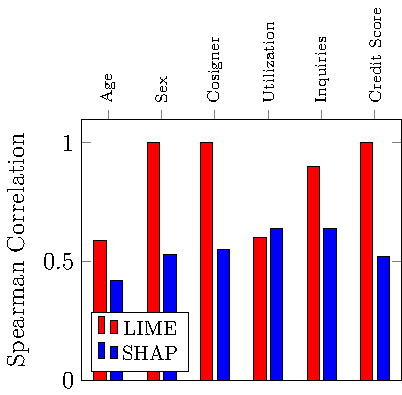
\includegraphics[width=\textwidth]{FinalFigures/sec4_3_perfect_data_sign_accs_final.pdf}
        \caption{Importance Sign Accuracy}
        \label{fig:perfect_data_model_acc}
        \end{subfigure}%
        %\hfill
        \begin{subfigure}{.3\textwidth}
        \centering
        %\fbox{\includegraphics[width=\textwidth,trim=0 10 70 70 mm, clip=true]{Figures/fig22.p}%{Final_Figures/fig21.png}
        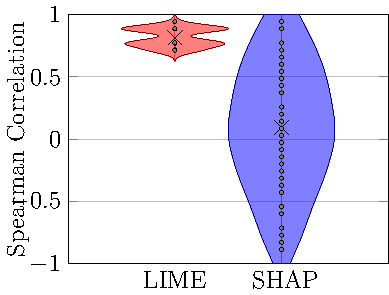
\includegraphics[width=\textwidth]{FinalFigures/sec4_3_perfect_data_spearmans_final.pdf}
        \caption{Importance Rankings}
        \label{fig:perfect_data_model_spearmans}
        \end{subfigure}
        \begin{subfigure}{.3\textwidth}
        \centering
        %\fbox{\includegraphics[width=\textwidth,trim=0 10 70 70 mm, clip=true]{Figures/fig22.p}%{Final_Figures/fig21.png}
        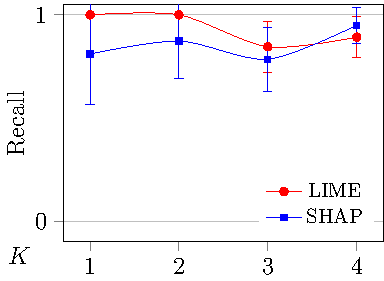
\includegraphics[width=\textwidth]{Figures/Final_Figures/sec4_3_perfect_data_recalls_final.pdf}
        \caption{Recall}
        \label{fig:perfect_data_model_recalls}
        \end{subfigure}
                \caption{LIME and SHAP when explaining an MLP with AUC $\sim .99$ trained a dataset with independent, and unconfounded features, and no unobserved features}
               \label{fig:perfect_data_model}
    \end{figure}
    
    
    
    
    
        \subsubsection{Ensuring that the Surrogate Model's Local Prediction is Correct} 
    \label{sec:e_fidelity}
        \begin{itemize}
        \item Since the underlying linear model of a LIME explanation is constructed to be a good representative of $\mathcal{M}$'s local behavior, it is natural to wonder whether the ability of a LIME explainer to correctly classify the label of the input being explained is related to the  quality of the explanation for that input.
    
        \item We only consider LIME here because LIME's surrogate model is a linear approximation of $\mathcal{M}$ and SHAP's is not; the idea of predictive accuracy makes sense for LIME and not SHAP. 
        
        \item For our experiment, we create a set of LIME explainers with different hyperparameters and, for 100 applicants, record whether they correctly classify the applicants' loan decision and the quality of their explanations for those applicants. 
    
        \item The results of our experiment suggest that ensuring that a LIME explainer correctly classifies the input being explained implies that the explainer deserves additional confidence.
    
                \begin{figure}[ht!]
                    \centering
                    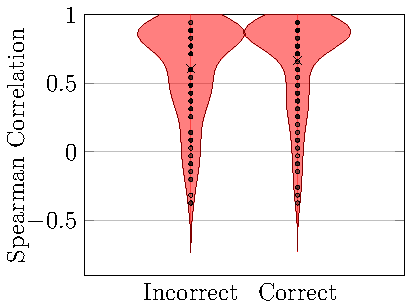
\includegraphics[width=.3\textwidth]{Figures/sec4_4_1pt_fid_spearmans.pdf}
                    \caption{Violin plots of Spearman correlations of feature rankings given by LIME explainers that did (right) and did not (left) correctly classify the input they were explaining}%Point plot for LIME's local fidelity versus its explanation quality, measured via Spearman rank correlation. Points indicate means and the vertical bars at each fidelity level indicate the 95\% confidence interval for the Spearman correlation taken over all the models that had that level of accuracy.}
                    \label{fig:lime_fidelity}
                \end{figure}
        \end{itemize}
    \subsection{Mitigation Strategies for Inconsistency} 
    \label{sec:inconsistency_mitigation}
         We address the issue of choosing a pipeline configuration by exploring whether it is worthwhile to use different forms of ensembles of explanations. 
    
        \subsubsection{Averaging Explanations Over Black Boxes}
        \begin{itemize}
            \item A straightforward way to address concerns about what black box to explain is to construct an average explanation over the black boxes one has available.
    
        \item Specifically, we repeat the experiments of Section \ref{sec:evaluating_faithfulness} twice, once with explanations of a single model and again with the modification that Spearman correlations are calculated between the ground truth and a feature ranking constructed by averaging feature importance values over LIME and SHAP explanations of 100 MLPs with ROC AUC at least $.9$.
    
       \item  It can be seen from Figures \ref{fig:mlp_increase} that averaging over increasing numbers of accurate MLPs benefits explanation quality somewhat and decreases the variance of the explanation quality. 
        \begin{figure*}[t!]
            \subfloat[Importance Sign Accuracy]{%
                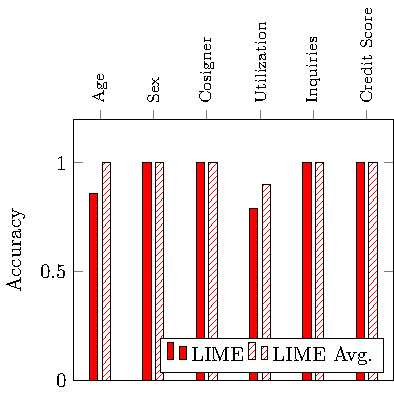
\includegraphics[width=.3\textwidth]{Figures/sec5_2_mlp_avg_lime_sign_accs.pdf}%
                \label{subfig:mlp_avg_lime_sign_accs}%
            }\hfill
            \subfloat[Importance Ranking]{%
                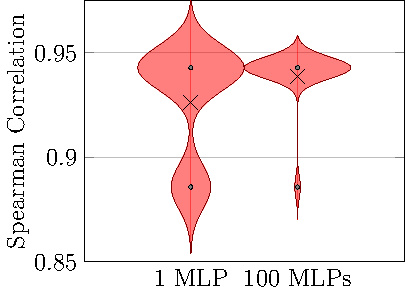
\includegraphics[width=.3\textwidth]{Figures/sec5_2_mlp_avg_lime_spearmans.pdf}%
                \label{subfig:mlp_avg_lime_spearmans}%
            }\hfill
            \subfloat[Recall]{%
                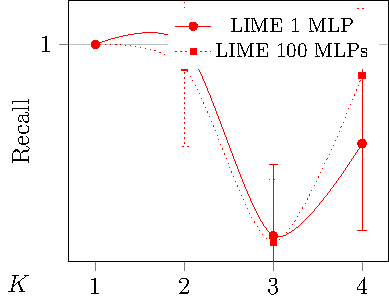
\includegraphics[width=.3\textwidth]{Figures/sec5_2_mlp_avg_lime_recalls.pdf}%
                \label{subfig:mlp_avg_lime_recalls}%
            }\\
            \subfloat[Importance Sign Accuracy]{%
                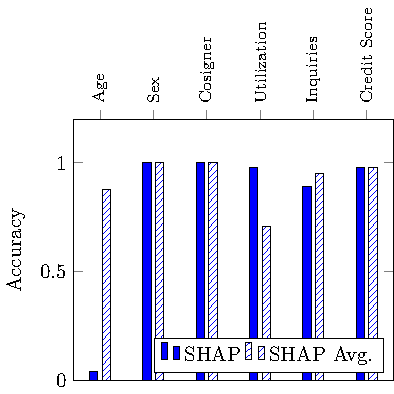
\includegraphics[width=.3\textwidth]{Figures/sec5_2_mlp_avg_shap_sign_accs.pdf}%
                \label{subfig:mlp_avg_shap_sign_accs}%
            }\hfill
            \subfloat[Importance Ranking]{%
                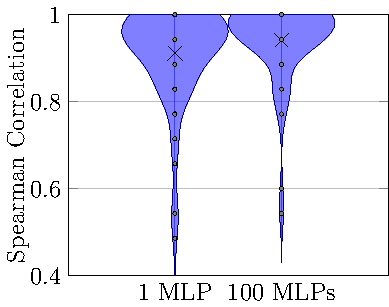
\includegraphics[width=.3\textwidth]{Figures/sec5_2_mlp_avg_shap_spearmans.pdf}%
                \label{subfig:mlp_avg_shap_spearmans}%
            }\hfill
            \subfloat[Recall]{%
                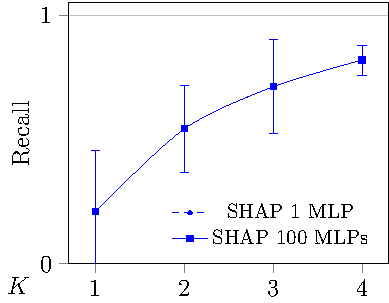
\includegraphics[width=.3\textwidth]{Figures/sec5_2_mlp_avg_shap_recalls.pdf}%
                \label{subfig:mlp_avg_shap_recalls}%
            }\\
            \caption{Relationships between numbers of MLPs used for averaging and explainer quality}
            \label{fig:mlp_increase}
        \end{figure*}
        \end{itemize}
    
    
        \subsubsection{Averaging Explanations Over Explainers}
            \label{sec:averaging_one_explainer}
            It is of interest whether the inconsistency of the explanations described in Section \ref{sec:conflict_between_within}, can actually be leveraged into an advantage. 

        \begin{itemize}
        \item  We do this by comparing the explanations of one LIME and the average explanation of 100 LIMEs for the prediction of an MLP on 100 applications. 
        
        \item Figure \ref{fig:lime_avg} shows that when averaging the explanations there is a slight benefit over using just one model. 
    
         \item Additional experiments using different explanation aggregation methods are provided in the Appendix. 
         \end{itemize}
    \begin{figure*}[!h]
    \centering
        \begin{subfigure}[t]{0.3\textwidth}
        \centering
        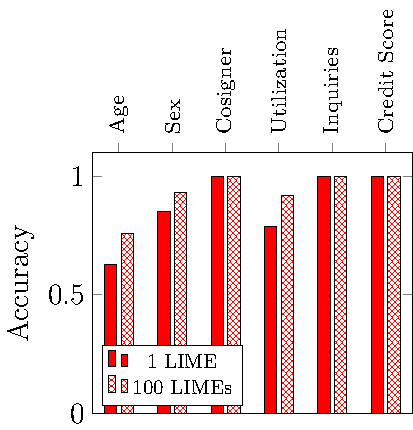
\includegraphics[width=\textwidth]{Figures/sec5_2_lime_avg2_sign_accs.pdf}
        \caption{Importance Sign Accuracy} \label{fig:lime_avg_sign_accs}
    \end{subfigure}\hfill
    \begin{subfigure}[t]{0.3\textwidth}
        \centering
        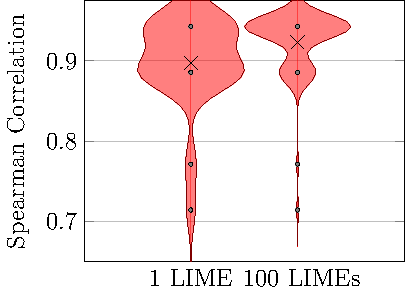
\includegraphics[width=\textwidth]{Figures/sec5_2_lime_avg2_spearmans.pdf}
        \caption{Importance Ranking} \label{fig:lime_avg_spearmans}
    \end{subfigure}\hfill
     \begin{subfigure}[t]{0.3\textwidth}
        \centering
        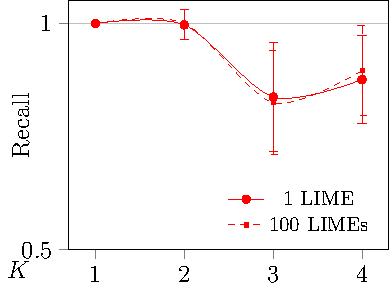
\includegraphics[width=\textwidth]{Figures/sec5_2_lime_avg2_recalls.pdf}
        \caption{Recall}
        \label{fig:lime_avg_recalls}
    \end{subfigure}
    \caption{Explanation quality when averaging over 100 LIME explainers of a single MLP}\label{fig:lime_avg}
    \end{figure*}
    
        
    
        \subsection{Summary and Discussion of Mitigation Strategies}
        \label{sec:summary_and_strategies}
            \begin{itemize}
            \item The results of our mitigation strategy experiments suggested that averaging the feature importance values of an ensemble of explanations was worthwhile when the ensemble consists of LIME explanations of different well performing black boxes, but not necessarily when the ensemble consists of explanations of the same black box. 
            
            \item Each explanation has two layers of approximation error with respect to the ground truth whereas each black box has only its own approximation error and captures different patterns in the training data. 
            
            \item Researchers who would like to investigate the importance and impact of features in a data generating process may find  exploring the following general strategy useful. 
            
            \paragraph{Stage 1}
                    \begin{itemize}
                        \item Pre-process data to remove correlated, confounded features\footnote{If the causal graph is available, Pearl's backdoor criterion can be used for this purpose. The causal graph can be estimated using Bayesian Networks if sufficient domain knowledge is available.}
                        \item Train $B$ black box models with minimal complexity and near optimal performance\footnote{Ideally, Rashomon sets of models would be constructed. However, at the time of writing, this is only possible for decision trees and GAMs.}
                    \end{itemize}
                
                % theoretical nalysis of LIME suggests that bandwidth should be big
            \paragraph{Stage 2}
                \begin{itemize}
                    \item For each black box model, obtain $E$ explainers%LIME explainers with high local fidelity.
                    \item Construct an average explanation by averaging the feature importance values over all $B\cdot E$ explanations. %LIME explanations.
                \end{itemize}

            \end{itemize}
    
    
\section{Case Study: Replicating Econometric Findings}
    \label{sec:case_study}
        To validate our claims and show how our mitigation strategies could be employed in practice, we will attempt to reproduce insights from an econometrics paper on home loan application approval \citep{bane2006econometric}. 

    To demonstrate the usefulness the general strategy outlined in Section \ref{sec:summary_and_strategies}, we will perform the following comparison. 
    
    \begin{tcolorbox}[title = Econometric Ground Truth Model $\mathcal{G}$]
    \begin{equation}
    \label{eqn:econ_gt}
    \begin{split}
        p(x) =\mathbf{\sigma}(.8 + 3.5\cdot \text{gdlin} + 4.7\cdot \text{typur} -4.4 \cdot \text{inson} - .4 \cdot \text{prop} -2.5 \cdot \text{unver} + .9 \cdot \text{fixadj} \\ - 1.4 \cdot \text{pubrec} - .9 \cdot \text{vr} - .03 \cdot \text{obrat} - .7 \cdot \text{old} + .8 \cdot \text{married} - .8 \cdot \text{gift})
    \end{split}
    \end{equation}
    \end{tcolorbox}
    %\subsection{Baseline Performance}
    %Figure \ref{fig:econ_cmp} compares the explanation quality  for 100 applicants from the baseline pipeline and recommended pipeline. %In the Appendix, we show also compare results for importance sign accuracy, Spearman rank correlation, and recall.

    Figure \ref{fig:econ_cmp} shows that our strategy performs at least as well as the baseline pipeline with respect to all three of our metrics. 

     
\begin{figure}[!h]
\centering
    \begin{subfigure}[t]{0.3\textwidth}
    \centering
    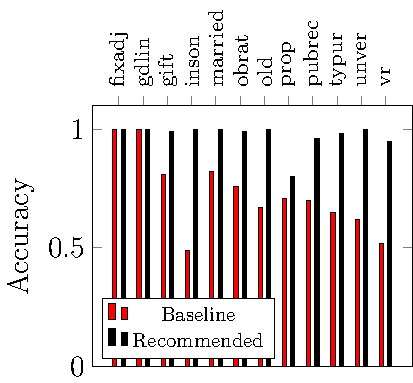
\includegraphics[width=\textwidth]{Figures/econ_cmp_sign_accs.pdf}
    \caption{Importance Sign Accuracy} \label{fig:econ_cmp_sign_accs}
\end{subfigure}\hfill
\begin{subfigure}[t]{0.3\textwidth}
    \centering
    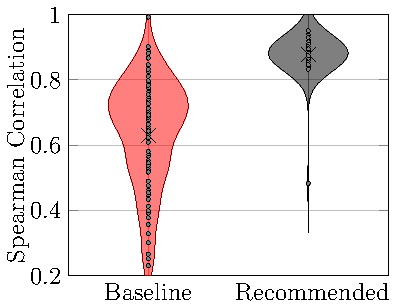
\includegraphics[width=\textwidth]{Figures/econ_cmp_spearmans.pdf}
    \caption{Importance Ranking} \label{fig:econ_cmp_spearmans}
\end{subfigure}\hfill
 \begin{subfigure}[t]{0.3\textwidth}
    \centering
    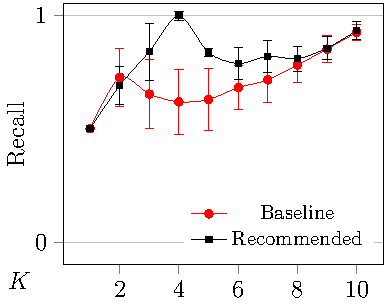
\includegraphics[width=\textwidth]{Figures/econ_cmp_recalls.pdf}
    \caption{Recall}
    \label{fig:econ_cmp_recalls}
\end{subfigure}
\caption{Improvements due to use of recommended pipeline instead of one without mitigations}\label{fig:econ_cmp}
\end{figure}
    

\section{Discussion and Conclusion}
    \label{sec:discussion}
    In this paper we have introduced and investigated issues of unfaithfulness and inconsistency of post hoc explainers and how they affect business research in particular. 

    \subsection{Summary of Findings and Take-away Messages}
        \begin{itemize}
        \item Using simulated loan application data sets, we produced ground truth application approval mechanisms $\mathcal{G}$ along with MLP approximators $\mathcal{M}$ trained on $\mathcal{G}$ and investigated how well popular post hoc explainers could produce correct insights into $\mathcal{G}$. 

        \item When evaluating the ability of the two most popular post hoc explainers, LIME and SHAP, to extract faithful insights from both real and simulated data, we identified the following issues that are cause for concern for researchers interested in $\beta$ estimation problems using post hoc explainers. 
        
        \item First, LIME and SHAP, cannot reliably extract the signs of the $\beta_i$ and cannot reliably rank features according to the feature ranking induced by $\beta$. 
        
        \item Second, users must deal with inconsistent explanations because not only do e.g. LIME and SHAP each produce different explanations for the same outcome, but LIME may produce self-contradictory explanations of the same outcome. 

        \item We propose that post-hoc explanations be viewed only as hypotheses can guide subsequent analyses after they are corroborated somehow. 

        \end{itemize}
    \subsection{On Mitigation Strategies}
        \begin{itemize}
        \item We proposed some intuitive mitigation strategies for the issues of unfaithful and inconsistent explanations. 
    
        \item To combat inconsistency, we proposed techniques to construct aggregate explanations that are better on average than individual explanations. 
        \end{itemize}

    \subsection{Guidance for Exploration of Strategies}
        \begin{itemize}
        \item The outline given in Section \ref{sec:summary_and_strategies} can undoubtably be improved and tailored to user-specific situations, and so is worth expounding. 
        
        \item During stage 1, before even beginning model development, users should attempt to understand the causal graph associated with their problems and employ statistical tests of unconfoundedness assumptions.

        \item Unless users are only interested in explaining a particular black box model, we propose that many be generated and used for explanations. 

        \item When starting stage 2, users should keep in mind the studies claiming that data scientists may misuse a post hoc explanation due to a fundamental misunderstanding of the explainer (by, e.g., having an incorrect understanding of what a Shapley value is) and/or inflicting their biases onto the explanation. 
        
        \item As we have discussed, due to the problems of unfaithfulness and inconsistency, researchers should not trust that a single explanation from any explainer applied to any black box model is true unless they can corroborate the explanation. 
        \end{itemize}

\subsection{Conclusion}
    Model-agnostic post hoc explainers certainly have legitimate use cases, but due to the nature of real business data sets and stakes associated with business problems, we urge the business community to use them with caution and with tempered expectations.

\bibliographystyle{informs2014}
\bibliography{refs}

\newpage

\end{document}
%%%%%%%%%%%%%%%%%

